\documentclass[12pt,a4paper,openright,twoside]{book}
\usepackage[utf8]{inputenc}
\usepackage{disi-thesis}
\usepackage{code-lstlistings}
\usepackage{notes}
\usepackage{shortcuts}
\usepackage{acronym}

\school{\unibo}
\programme{Corso di Laurea Magistrale in Ingegneria e Scienze Informatiche}

\title{EleKtion: \\
libreria Kotlin Multiplatform \\
per la democrazia digitale  \\
in nuovi contesti
}
\author{Jacopo Corina}
\date{\today}
\subject{Laboratorio di sistemi software}
\supervisor{Prof. Danilo Pianini}
\session{III}
\academicyear{2022-2023}

% Definition of acronyms
\acrodef{IoT}{Internet of Thing}
\acrodef{vm}[VM]{Virtual Machine}

\acrodef{gh}[GH]{GitHub}

\acrodef{gha}[GH Actions]{GitHub Actions}

\acrodef{ghp}[GH Pages]{GitHub Pages}

\acrodef{ci}[CI]{Continuous Integration}

\acrodef{cd}[CD]{Continuous Delivery}

\acrodef{dsl}[DSL]{Domain Specific Language}
\acrodef{f1}[F1]{Formula 1}

\acrodef{npm}[NPM]{Node Package Manager}

\acrodef{jvm}[JVM]{Java Virtual Machine}


\mainlinespacing{1.35} % line spacing in mainmatter, comment to default (1)

\begin{document}

\frontmatter 
\frontispiece

\begin{abstract}	
Max 2000 characters, strict.
\end{abstract}

\begin{dedication} % this is optional
Ai miei genitori
\end{dedication}

%\begin{acknowledgements} % this is optional
%Optional. Max 1 page.
%\end{acknowledgements}

%----------------------------------------------------------------------------------------
\tableofcontents   
\listoffigures     % (optional) comment if empty
\lstlistoflistings % (optional) comment if empty
%----------------------------------------------------------------------------------------

\mainmatter

%----------------------------------------------------------------------------------------
\chapter{Introduzione}
\label{chap:introduction}
%----------------------------------------------------------------------------------------
\chapter{Democrazia digitale}
Il termine \textit{Democrazia}, derivante dal greco \textit{governo del popolo},
indica un forma di governo nella quale il potere appartiene al popolo ed è esercitato attraverso forme dirette, che coinvolgono attivamente
i cittadini, e attraverso forme rappresentantive, che prevedono un sistema di rappresentanza, la quale viene rinnovata ciclicamente
attraverso apposite elezioni.

In una qualunque forma di \textit{democrazia}, sono fondamentali le basi dei principi di elezioni libere in cui i cittadini sono considerati equi, partecipazione
attiva dei cittadini alla vita politica, protezione dei diritti fondamentali e della libertà personale attraverso costituzioni \cite{vinod2017state}.

Nelle epoche successive alle prime forme di democrazia "unanime" (per quanto il concetto di cittadinanza fosse assai diverso da quello attuale,
ad esempio, erano escluse donne, schiavi e minori di 20 anni), complice anche la complessità
delle materie da amministrare e il numero dei partecipanti fisici, la democrazia
rappresentativa ha preso la maggior diffusione. 

La modernizzazione tecnologica, accelerata di recente con l'avvento della pandemia da Covid-19 che ha evidenziato notevole problemi
logistici, tra cui la gestione del distanziamento \cite{sotoacosta} e ha aperto un ventaglio di possibilità tali da
permettere un ritorno ad un controllo più diretto da parte della collettività.

La \textit{democrazia digitale} (o \textit{e-democracy}) è definibile come "l'esercizio di processi decisionali democratici attraverso 
l'uso di informazioni e tecnologie abilitanti alla comunicazione, in particolare Internet"\cite{rotzocki}.

Queste tecnologie, abilitanti a rompere i vincoli geo-fisici e territoriali,
permettono di facilitare l'esercizio di ulteriori forme di democrazie,
come quella partecipata, in cui i cittadini, piuttosto che
sostituirsi ai rappresentanti, forniscono idee sullo sviluppo dell'indirizzo di governo
permettendo così di creare un collettore di confronto ed analisi di situazioni differenti.

Tuttavia, è necessario considerare che un uso eccessivamente estensivo di questi strumenti
può portare al rischi di coinvolgere persone che non hanno abbastanza competenze relativamente 
a temi delicati, ad esempio le politiche sociali. 

Inoltre, nonostante la virtualizzazione della partecipazione permette alle fasce più disagiate di essere
maggiormente coinvolte, introduce un motivo di scetticismo relativamente alla componente tecnologica
in ambito di sicurezza informatica, usabilità, segretezza e manipolazione del voto \cite{aichholzer2020experience}.

Stabilire un legame di fiducia con queste tecnologie, normarne la verificabilità, stabilire principi di 
\textit{accountability}, sono i fattore principali e quindi una pre-condizioni essenziali
per la loro diffusione. 
Alcuni autori (\cite{mcgaley}) sostengono che è impossibile avere leggitimità in quanto "la natura dei computer è tale che il loro funzionamento interno è segreto.
Poiché le transazioni e i calcoli avvengono a livello elettronico, 
non è fisicamente possibile per gli esseri umani osservare esattamente ciò che un computer sta facendo."

L'applicazione più comune di queste tecnologie emergenti è legata al mondo della politica\cite{aichholzer2020experience}:
sono degni di nota casi come l'Estonia, che dal 2005 rende possibili via Internet le votazioni
per elezioni e referendum, e l'Islanda che tramite un ambizioso progetto tenta di riscrivere %qualche esempio in piu
la costituzione con l'apporto dei cittadini. In Italia possiamo rilevare l'applicativo PartecipaMi,
organizzata per mettere in contatto la popolazione milanese con l'amministrazione comunale.\cite{WebsitePartecipaMi}

Inoltre, queste soluzioni sono spesso adottate da partiti o movimenti politici per avviare iniziative
e votazioni interne tra i membri, come nel caso del Partito Pirata tedesco in Germania (piattaforma LiquidFeedback),
o il Movimento 5 Stelle in Italia (piattaforma Rousseau). Lo scopo principale è quello di promuovere la discussione
di proposte tra i membri di un organizzazione, le quali saranno portate in sede legislativa da un loro rappresentante\cite{korthagen2020non}.

Sistemi come LiquidFeedback, OpenDCN, Airesis, essendo strutturati come applicativi end-to-end,
pongo molta enfasi sull'interazione tra utenti, la presentazione e validazione di proposte,
l'eventuale presenza di deleghe, l'espressione del voto tramite una lista di preferenze, ma
non permettono la variazione delle logiche di selezione del vincitore da applicare\cite{Trapanese:2018}.

In altri, una fase di analisi iniziale poco trasversale ha portato a dar maggior risalto
ad aspetti non funzionali, come la privacy, rispetto a quelli funzionali come il modello di democrazia
da applicare, che per alcuni aspetti rimane implicito\cite{Pianini:2019}.
Ciò è dovuto anche al fatto che il maggior coinvolgimento si concentra 
principalmente alle fasi iniziali e finali del ciclo di votazione \cite{hennen2020european}.
La mancanza di elementi formalizzanti, che descrivono dettagliatamente tutti gli step applicati nel
processo, unita alle variazioni ed evoluzioni che vengono apportate nel tempo, portano alla divergenza di \textit{logica del flusso} rispetto all'idea iniziale, 
che conseguentemente non risulterà chiara agli utilizzatori e potenzialmente potrebbe scoraggiare l'utilizzo della piattaforma\cite{Pianini:2019}.



Al di là dell'applicazione di e-democracy nel mondo della politica, che riscontra
ostacoli più legati all'aspetto organizzativo e umano, che all'aspetto tecnico,
vi sono esempi notabili anche nel campo della digitalizzazione pervasiva, ad esempio nell'ambito delle \textit{smart cities}.
Ricollegandosi al fenomeno dei cambiamenti climatici che stanno inesorabilmente continuando a proliferare,
in certe zone del mondo l'acqua potabile sta diventando un bene sempre meno reperibile e se sempre più da salvaguardare.
\cite{smartwater} pone il focus sull'adozione di sistemi di "IdroInformatica". Questo tipo di sistemi permettono di analizzare 
e monitorare, attraverso sensori e sistemi real-time SCADA (Supervisory Control And Data Acquisition), gli attuali flussi e pressioni nella
rete di distribuzione ed effettuare predizioni sui futuri guasti. Questi strumenti di analisi possono fornire ai cittadini
informazioni su come ottimizzare l'utilizzo delle risorse. L'unione di questi sistemi, ad una politica di gestione elettronica e democratica
che porti a prendere parte alle decisioni per i cambiamenti che coinvolgono il regime di gestione presente in una determinata area,
permetterebbe una miglior localizzazione circa le soluzioni da intraprendere, ed ai cittadini una maggior consapevolezza, in quanto sono i principali \textit{stakeholders} 
e a loro viene attribuito anche un principio di responsabilità.
In altri Stati, come Canada e Paesi Bassi, la gestione dell'acqua è delegata ad un gestione locale, che promuove la collaborazione tra soggetti pubblici e privati.

Questi nuovi approcci alla gestione democratica degli interessi dei cittadini aprono nuovi
scenari di trasparenza e fiducia reciproca, permettendo un maggior capacità espressione di espressione
verso i rappresentanti ma anche da parte di chi è ora in grado di percepire, in ottica di miglioramento continuo,
le esigenze del mondo "reale". 
L'intermediazione, applicata a questi nuovi contesti, continua a rimanere essenziale.
Piuttosto che diventare un nuovo "medium" per imporre decisioni, risulta più efficace per
favorire lo scambio costruttivo, mantenendo comunque le opportune autonomie riguardo alle
decisioni finali, tutelando gli interessi collettivi e al contempo educando le persone a mantenere
la libertà di pensiero\cite{castelfranchi2019problematic}.
%strumento utile per mettere al centro dell'attenzione il cittadino ma deve essere mantenuto il rapporto bilaterale
%articolo rino
%Seppur aventi regole simili in taluni casi, ciascuno sport è influenzato da molti fattori:
%i concorrenti, gli ambienti di gara, i tifosi, e altri aspetti, che contribuiscono a rendere 
%ogni campionato come un capitolo a sè stante. 
%Non per ultimo, ognuno di essi ha un proprio metodo di calcolo ed organizzazione delle competizioni. 
%Soprattutto in caso di pareggi, è opportuno avere una logica per risolvere il conflitto e determinare un ordine specifico per
%le classifiche. Se si considerasse l'esito di ciascuna gara come un votazione, cambiando
%l'algoritmo utilizzato per un campionato, si otterrebbero esiti differenti, o ancora,
%se si cambiasse la logica di vittoria nelle fasi di un campionato, si potrebbe simulare come
%sarebbe stato l'esito finale con regole differenti.
%modello implicito, sforzi iniziali ma analisi poco dettagliata lascia punti scoperti, si da maggior risalito a req non funzionali che funzionali
%aumentare curva apprendimento e incertezza aumenta con il numero di funzionalità e impatto negativo sull' usabilità

%----------------------------------------------------------------------------------------

%----------------------------------------------------------------------------------------
\chapter{Analisi}
In questo capitolo verrà descritta l'analisi sugli aspetti che dovranno 
caratterizzare la libreria multipiattaforma \texttt{EleKtion}.

Verrà esposto un approfondimento sui tipi di voto
ed alcuni algoritmi applicabili per ciascun tipo; successivamente sarà definito un 
elenco di requisiti che dovranno essere considerati nelle fasi successive e infine,
sarà fornita una modellazione del dominio mediante diagramma UML.
\section{Voto a singola preferenza}
La tipologia di voto a singola preferenza impone al votante di effettuare una scelta tra un
numero definito di concorrenti. Al termine della votazione, tipicamente si adotta il criterio
della votazione maggioritaria: si contano i voti ottenuti da ciascun concorrente, e colui che ottiene il
numero più elevato, risulta vincitore. A seconda del contesto preso in considerazione,
è possibile avere più turni per diminuire di volta in volta il numero di concorrenti coinvolti.
Se si arriva ad un pareggio, è possibile effettuare un nuovo ballottaggio oppure adottare
criteri secondari, che variano in base al dominio trattato.
\section{Voto a lista di preferenze}
La tipologia di voto a lista di preferenze non impone al votante di effettuare un'unica scelta,
bensì di fissare un ordinamento tra i concorrenti che parta dal meno preferito al più preferito
o viceversa. Questa logica permette di conservare più contenuto informativo sulle preferenze
rispetto alla singola scelta, e offre anche una panoramica di gradimento degli altri concorrenti.
Questo tipo di voto è stato introdotto inizialmente dall'algoritmo di Condorcet ed adottato
anche nelle sue varianti. Di seguito viene data una spiegazione sul funzionamento dell'algoritmo
di Condorcet, e di un suo derivato, l'algoritmo di Schultze.
\subsection{Algoritmo di Condorcet}
L'algoritmo di Condorcet permette di estrarre un vincitore tra ${n}$ concorrenti,
applicando il criterio di maggioranza nei confronti tra le coppie di concorrenti.
Si generano le possibili coppie, si confrontano e si valuta quale coppia ha ottenuto il
maggior numero di preferenze. Nello scontro a coppie, un concorrente è vincitore se in un
voto occupa una posizione preferenziale rispetto all'altro.

Di seguito viene riportato un esempio, supponendo di avere tre possibili concorrenti, A, B, C,
e 60 differenti votanti, che ordinano i concorrenti dalla posizione 1 alla posizione 3 dove la posizione 1 
indica la posizione di maggior preferenza.
Si ottengono delle liste di preferenze come rappresentato in tabella \ref{table:voticondorcet}, in cui
è mostrata l'occorrenza di ciascuna lista.

\renewcommand{\arraystretch}{1.5}
\begin{table}[H]
    \centering
    \begin{tabular}{|c|c|c|c|}
    \hline
    \multicolumn{1}{|l|}{Posizione 1} & \multicolumn{1}{|l|}{Posizione 2} & \multicolumn{1}{|l|}{Posizione 3} & \multicolumn{1}{l|}{Numero di occorrenze della lista } \\ \hline
    A & C & B & 23                              \\ \hline
    B & C & A & 19                              \\ \hline
    C & B & A & 16                              \\ \hline
    C & A & B & 2                               \\ \hline
    \end{tabular}
    \caption{Tabella delle liste di preferenze, con l'occorrenza di ciascuna lista}
    \label{table:voticondorcet}
\end{table}

Ora è possibile effettuare confronti tra le coppie, partendo ad esempio dalla coppia (B,C)
\begin{itemize}
    \item{Nella prima lista C è in una posizione favorevole rispetto a B, quindi C ottiene 23 punti}
    \item{Nella seconda lista B è in una posizione favorevole rispetto a C, quindi B ottiene 19 punti}
    \item{Nella terza lista C è in una posizione favorevole rispetto a B, quindi C ottiene 16 punti}
    \item{Nella quarta lista C è in una posizione favorevole rispetto a B, quindi C ottiene 2 punti}
\end{itemize}

Si ha che il concorrente C batte il concorrente B con un punteggio di 41 a 19.

Facendo i confronti tra le coppie (A,B) e (A,C) si ottiene che il concorrente
B batte il concorrente A con un punteggio di 35 a 25, e il concorrente C batte il concorrente
A con un punteggio di 37 a 23. Il risultato finale è quindi il seguente:
\begin{itemize}
    \item{Posizione 1: C}
    \item{Posizione 2: B}
    \item{Posizione 3: A}
\end{itemize} 

In alcuni casi il metodo di Condorcet può non portare ad alcun vincitore, in quel caso si
ha un ciclo, ad esempio, trovandosi in una situazione 
in cui C $>$ B, B $>$ A, A $>$ C.

Le varianti del metodo di Condorcet ottimizzano l'algoritmo per minimizzare il rischio
di indeterminazione del vincitore.
Può accedere, in Condorcet come nelle sue varianti, di ottenere dei pareggi,
i quali avvengono quando due o più concorrenti pareggiano l'uno con l'altro ma 
battono tutti i restanti. La situazione di pareggio può essere gestita in vari
modi, ad esempio, estraendo una sequenza in modo casuale, valutando altri criteri
come la preferenza nei singoli voti (most first choice) oppure mantenendo il set di pareggio
senza effettuare alcuna azione.

Dato il risultato della votazione, è possibile definire l'utilità individuale come il grado
di soddisfazione del votante. Il grado di soddisfazione sarà tanto più alto 
quanto più vicino è il risultato rispetto al voto espresso.

Concludendo, l'algoritmo porta ad un risultato nel quale si tende a massimizzare
l'utilità per il maggior numero di votanti, ossia a massimizzare l'utilità
complessiva. 

\subsection{Algoritmo di Schultze}
L'algoritmo di Schultze, conosciuto anche come Schwartz Sequential Dropping (SSD),
è una variante di Condorcet basata sulla sommatoria del conteggio delle preferenze tra i concorrenti.

Ad esempio, nel caso in cui si hanno 3 candidati, A, B, C,
e questi vengono ordinati in una lista di preferenze dalla posizione 1 alla posizione 3 dove la posizione 1 
indica la posizione di maggior preferenza, si può avere il seguente risultato:
\begin{itemize}
    \item{Posizione 1: A}
    \item{Posizione 2: B}
    \item{Posizione 3: C}
\end{itemize}    
In questa lista A ottiene 2 punti, B ottiene 1 punto mentre C nessuno.

Riprendendo la situazione presente in tabella \ref{table:voticondorcet} e moltiplicando
i punti per il numero di occorrenze della lista, si ha un totale dei punti pari a 48
per la lista in oggetto. Proseguendo con l'algoritmo, la situazione finale è mostrata in tabella \ref{table:risultatischultze}

\begin{table}[H]
    \centering
    \begin{tabular}{|c|c|c|c|c|c|}
    \hline
    \multicolumn{1}{|l|}{concorrente} & \multicolumn{1}{|l|}{x 23} & \multicolumn{1}{|l|}{x 19} & \multicolumn{1}{l|}{x 16} & \multicolumn{1}{l|}{x 2} & \multicolumn{1}{l|}{Sommatoria} \\ \hline
    A & 2 & 0 & 0 & 1 & 48                              \\ \hline
    B & 0 & 2 & 1 & 0 & 54                              \\ \hline
    C & 1 & 1 & 2 & 2 & 78                             \\ \hline
  
    \end{tabular}
    \caption{Tabella delle sommatorie ottenute con l'applicazione dell'algoritmo di Schultze}
    \label{table:risultatischultze}
\end{table}

Prendendo in considerazione le sommatorie in ordine decrescente, otteniamo, il seguente risultato:
\begin{itemize}
    \item{Posizione 1: C}
    \item{Posizione 2: B}
    \item{Posizione 3: A}
\end{itemize} 

Il risultato di Schultze non coincide sempre con il risultato di Condorcet.

\newpage
\section{Requisiti}
La libreria \texttt{EleKtion} fornirà la possibilità di creare ed effettuare votazioni.
Essa non tratterà la parte preliminare ad una votazione, quale fase di proposta, discussione,
eventuali pre-votazioni o quorum, ma porrà l'obiettivo sulla definizione e gestione dei concorrenti coinvolti,
la tipologia di algoritmo utilizzato per ottenere il risultato finale ed i voti presenti nella fase di votazione.
Al termine della stessa, sarà disponibile una classifica che riporta informazioni 
circa le specifiche impostate e le caratteristiche dei concorrenti.


Ciascuna votazione avrà associata una competizione con un metrica che caratterizza l'operato del concorrenti.
Prendendo esempi di riferimento legati al mondo del \textit{motor sport},
si potrebbe pensare ai punti totalizzati per ogni gara, come nel caso di \textit{\ac{f1}} o \textit{Moto GP}.

Seppur in molti casi le regole non cambiano in modo drastico, ciascuno sport è influenzato da molti fattori:
i concorrenti, gli ambienti di gara, i tifosi, e altri aspetti, che contribuiscono a rendere 
ogni campionato come un capitolo a sè stante. 

Non per ultimo, ognuno di essi ha un proprio metodo di calcolo ed organizzazione delle competizioni. 
Soprattutto in caso di pareggi, è opportuno avere una logica per risolvere il conflitto e determinare un ordine specifico per
le classifiche. 
Se si considerasse l'esito di ciascuna gara come un votazione, cambiando
l'algoritmo utilizzato in un campionato, si otterrebbero esiti differenti, o ancora,
se si cambiasse la logica di vittoria nelle fasi di un campionato, si potrebbe simulare come
sarebbe stato l'esito finale con regole differenti.

    \subsection{Requisiti funzionali}
    \begin{itemize}
        \item{Definizione di un gestore di votazioni, intesi come contenitore delle stesse. Ciascuna votazione
        dovrà essere indipendente dalle altre. L'eventuale collegamento tra le stesse sarà demandato all'utilizzatore della libreria.}
        \item{Definizione dei concorrenti che rappresenteranno i candidati disponibili, delle relative caratteristiche e di
        eventuali punteggi, che potranno essere presenti a seconda del dominio della votazione.
        Gli eventuali punteggi saranno collegati ad una specifica metrica di interesse.
        }
        \item{Definizione dell'algoritmo da utilizzare. L'algoritmo dovrà determinare la logica con cui saranno
        confrontati e selezionati i concorrenti. L'algoritmo potrà utilizzare la metrica disponibile per
        effettuare ulteriori valutazioni in occasione di pareggio o altre casistiche definibili dall'utilizzatore.
        L'algoritmo potrà essere parametrizzato, per impattare il proprio funzionamento.   }
        \item{Definizione dei voti presenti nella votazione. La tipologia di voto dovrà essere dipendente dall'algoritmo utilizzato,
        e in ogni caso potrà essere dei seguenti tipi:
        \begin{enumerate}
            \label{tipidivoto}
            \item{Voto a singola preferenza}
            \item{Voto a lista di preferenze}
        \end{enumerate}

        Dovrà essere data la possibilita si anonimizzare il votante, in modo tale che successivamente non sia possibile risalire al suo identificativo.

        
        }
        \item{Le fasi di definizione dovranno essere correlate ad opportuni controlli di congruità, al fine di elaborare la votazione in modo coerente.}
        \item{La classifica finale dovrà essere disponibile e visualizzabile dall'utilizzatore. Dovrà esser data evidenza
        di eventuali situazioni di pareggio, di quale algoritmo è stato utilizzato e delle caratteristiche dei concorrenti.}
    \end{itemize}
    \subsection{Requisiti non funzionali}
    \begin{itemize}
        \item{Dovrà essere possibile definire tutti gli elementi necessari attraverso l'uso di costrutti che agevolino la rapidità di creazione,
        evitando che l'utilizzatore effettui manualmente i controlli minimi ed obbligatori.}
    \item{La libreria dovrà essere disponibile su molteplici piattaforme, facilmente importabile in esse ed avere una documentazione
    a corredo.}
    \end{itemize}


\section{Modello del dominio}
\label{modellodominio}
\texttt{EleKtion} avrà a disposizione uno o più gestori di votazioni. 
I gestori sono indipendenti tra loro e così anche le votazioni all'interno degli stessi,
fatto salvo l'uso coerente della tipologia di votazione e della metrica di punteggio,
che rimane stabile in ogni gestore.

Non è contemplata l'ipotesi di più turni nella stessa votazione, 
quindi in tal caso dovranno essere gestiti come votazioni separate.

Una votazione avrà associata una determinata competizione, 
alla quale è associato l'elenco dei concorrenti. 

Ciascun concorrente può avere una serie di punteggi,
 e la tipologia di punteggio è strettamente collegato alla tipologia di competizione.

La votazione, inoltre, ha associato l'elenco dei voti,
i quali hanno riferimento sia del votato che del votante,
in caso di votazione non anonima.
È importante che un voto, per essere considerato valido, 
sia riferito ad un candidato esistente e sia della tipologia ammessa dalla votazione.

Infine, ci può essere un solo algoritmo collegato alla votazione,
il quale può contenere dei parametri per effettuare variazioni nella configurazione per il suo funzionamento.
La votazione avrà un' unica classifica finale, la quale può essere consultata.

In figura \ref{fig:modellodominio} viene rappresentato il diagramma UML con le interfacce che modellano
il dominio descritto in questo capitolo.
\newpage

\begin{figure}
   \centering
    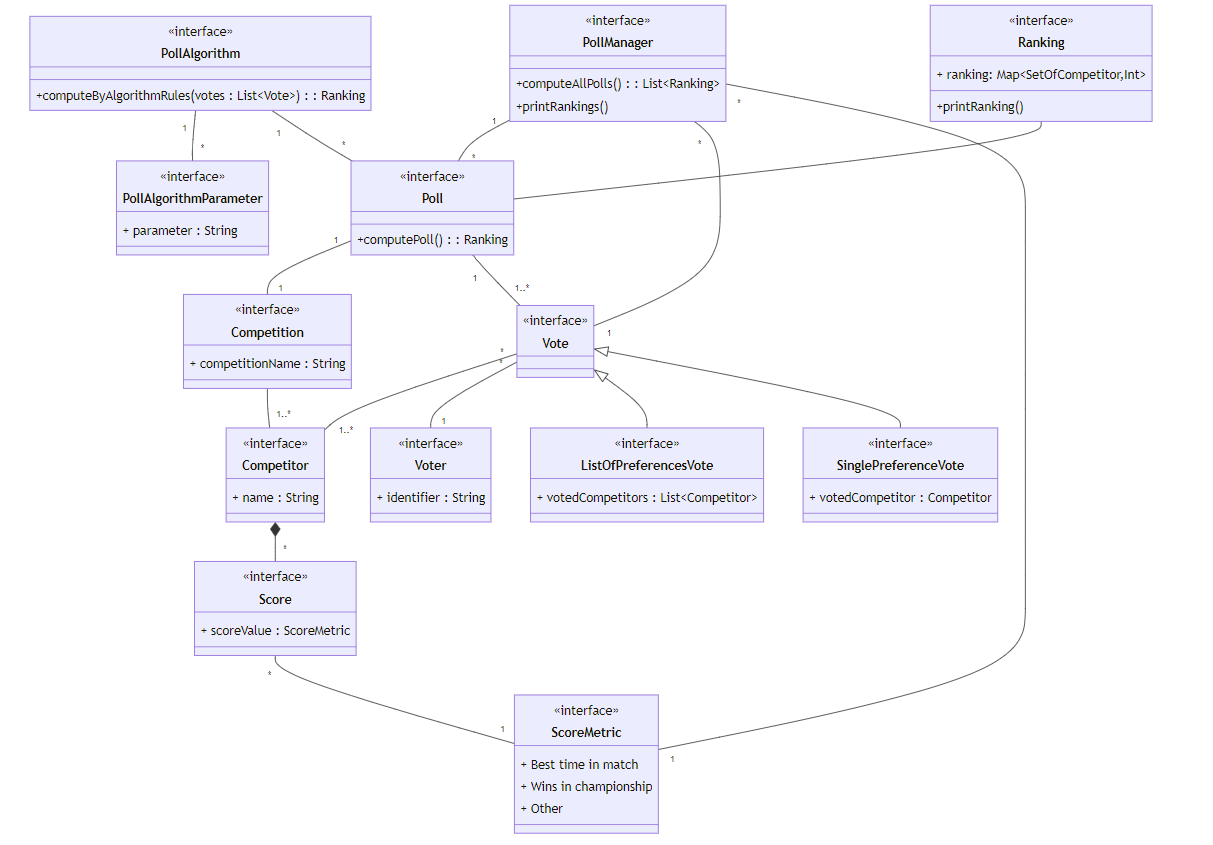
\includegraphics[width=1.1\linewidth]{figures/modellodominio.png}
    \caption{Diagramma UML del modello di dominio di \texttt{EleKtion}}
   \label{fig:modellodominio}
\end{figure}

%----------------------------------------------------------------------------------------
\chapter{Design}
In questo capitolo, partendo dalla modellazione del dominio descritta nel capitolo \ref{modellodominio}, 
sarà sviluppato un approfondimento sulla definizione delle metriche di punteggio e sulla porzione
impattata dall'introduzione di \ac{dsl}, volto al miglioramento dell'utilizzabilità della libreria \texttt{EleKtion}.
Per ciascuna funzionalità verrà evidenzata un'apposita descrizione e un diagramma UML
che esplichi come saranno organizzate le interfacce e le classi astratte.

Questi diagrammi sono realizzati con il presupposto di poter adottare l'utilizzo
dei seguenti costrutti:
\begin{itemize}
\item{Tipi \texttt{generici} \cite{WebsiteKotlinGenerics};}
\item{\texttt{Overloading} degli \texttt{operatori} \cite{WebsiteKotlinOperatorOverloading};}
\item{\texttt{Higher order functions} (in particolare \texttt{function literal with receiver}) \cite{WebsiteKotlinLambda};}
\item{\texttt{Companion object} \cite{WebsiteKotlinCompanionObject}.}
\end{itemize}

Si rimanda alle fonti per l'approfondimento specifico in \texttt{Kotlin}, la sintassi utilizzata nei diagrammi
è generica ed astrae dal linguaggio specifico.


\section{Domain Specific Language per la definizione del gestore di votazioni }
Questo \ac{dsl} è pensato per facilitare la creazione del gestore di votazioni.
Un gestore di votazioni viene vincolato ad adottare uno specifico tipo \texttt{S}, sottotipo di \texttt{ScoreMetric}, ed uno specifico
tipo di voto \texttt{V}, sottotipo di \texttt{Vote}.

Una metrica è definibile come il criterio tale per cui un concorrente può essere messo a confronto con un altro, sulla base della
sua prestazione nella competizione. Pertanto, è rappresentabile come una comparazione tra valori.
Dall'interfaccia \texttt{ScoreMetric} possono essere definiti numerosi sottotipi utili alla competizione trattata, ad esempio il punteggio di un concorrente
può essere legato ai punti assegnati in una gara, alle vittorie ottenute in campionato, oppure a criteri legati al tempo.
Per facilitarne la creazione è utile definire una funzione di supporto contenuta in un \texttt{companion object}, come mostrato in figura \ref{fig:metrica}.

\vfill
\begin{center} 
\begin{figure}[H]
    \centering
     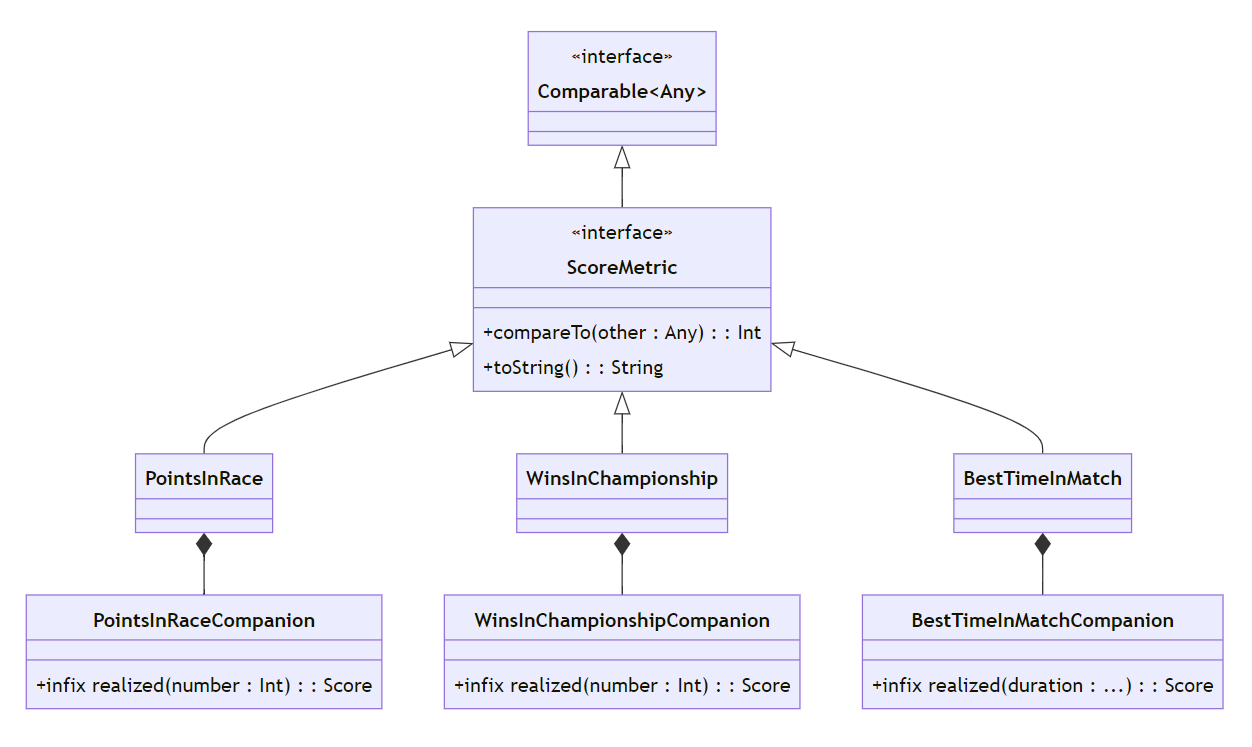
\includegraphics[width=1.1\linewidth]{figures/scoremetric.PNG}
     \caption{Diagramma UML dell'organizzazione di una metrica}
    \label{fig:metrica}
 \end{figure}
\end{center}
\vfill

I tipi \textit{S} e \textit{V} vincolano i seguenti componenti che verranno trattati, pertanto non è possibile adottare diversi metriche di punteggio tra i concorrenti,
o diversi tipologie di voto, tra le varie votazioni presenti nel medesimo gestore.

Il punto di ingresso dell'intero flusso è rappresentato dalla funzione \texttt{initializedAs}, al suo interno è possibile inizializzare una votazione attraverso 
la funzione \texttt{poll}, e l'utilizzo dell'operatore unario \texttt{+}, per l'aggiunta di quest'ultima alla lista di votazioni.
In figura \ref{fig:pollManagerDSL} viene mostrato il diagramma UML delle interfacce e della classe astratta.
\vfill
\begin{center} 
\begin{figure}[H]
    \centering
     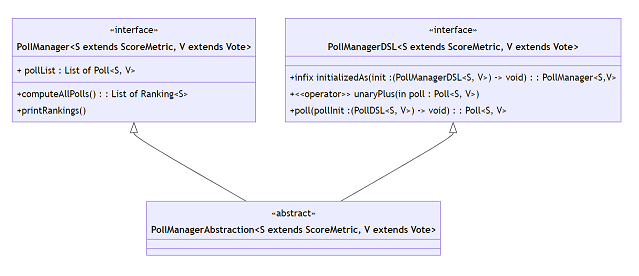
\includegraphics[width=1.1\linewidth]{figures/pollManagerDSL.png}
     \caption{Diagramma UML del \ac{dsl} per la definizione del gestore di votazioni}
    \label{fig:pollManagerDSL}
 \end{figure}
\end{center}
\vfill
 \newpage


 \section{Domain Specific Language per la definizione della votazione}
 Questo \ac{dsl} è pensato per facilitare la creazione di una votazione.
 In una votazione è obbligatorio scegliere l'algoritmo con cui sarà elaborato l'esito, 
 l'algoritmo può ricevere parametri utili al uso funzionamento, attraverso l'utilizzo dell'
 operatore unario \texttt{+} presente in \texttt{PollAlgorithmDSL}.
 In base al tipo di voto (vedi capitolo \ref{tipidivoto}) è utile definire un costrutto
 per agevolarne la creazione.
 Nel caso in cui il voto sia a singola preferenza, è necessario specificare
 l'identificativo del votato e l'identificativo del votante (vedi funzione \texttt{votedBy} in \texttt{SPVoteAlgorithmDSL}, figura \ref{fig:pollAlgorithmDSL}). Nel caso in cui quest'ultimo non 
 sia richiesto, corrisponderà ad un identificativo casuale (vedi funzione \texttt{asAnonymousVote} in \texttt{SPVoteAlgorithmDSL}, figura \ref{fig:pollAlgorithmDSL}).
 Nel caso in cui il voto sia a lista di preferenze, per costruire la lista è necessario specificare l'elenco degli identificativi dei votati,
 utilizzando la funzione \texttt{then} in concatenazione (vedi funzione \texttt{then} in \texttt{LOPVoteAlgorithmDSL}, figura \ref{fig:pollAlgorithmDSL})).
 Allo stesso modo del voto a singola preferenza, è prevista la possibilità di anonimizzare il votante.
 Come visibile in figura \ref{fig:pollAlgorithmDSL}, sono previsti metodi per semplificare l'inizializzazione dei possibili algoritmi:
 \begin{itemize}
    \item{\texttt{majorityVotesAlgorithm}: rappresenta la creazione di un algoritmo a maggioranza, in cui il vincitore è colui che ricevuto più voti;}
    \item{\texttt{majorityVotesHScoreAlgorithm}: rappresenta la creazione di un algoritmo a maggioranza, in cui il vincitore è colui che ricevuto più voti.
    Se si verificano pareggi, viene selezionato il concorrente che ha il punteggio maggiore, secondo la metrica di punteggio definita;}
    \item{\texttt{majorityVotesHScoreAlgorithm}: rappresenta la creazione di un algoritmo a maggioranza, in cui il vincitore è colui che ricevuto più voti.
    Se si verificano pareggi, viene selezionato il concorrente che ha il punteggio minore, secondo la metrica di punteggio definita;}
    \item{\texttt{condorcetAlgorithm}: rappresenta la creazione dell'algoritmo di Condorcet;}
    \item{\texttt{schultzeAlgorithm}: rappresenta la creazione dell'algoritmo di Schultze.}
 \end{itemize}

 In figura \ref{fig:pollDSL} vengono mostrati gli altri metodi utili alla creazione di una votazione:
 La funzione \texttt{competition}, utile alla creazione della competizione,
 richiede che venga definito un nome alla competizione e un inizializzatore in cui saranno definiti i concorrenti.
 Quest'ultimo, così come l'algoritmo desiderato, sono effettivamente assegnati alla votazione
 attraverso l'uso dell'operatore unario \texttt{-}.
 Infine è possibile aggiungere un elenco di voti, preferibilmente creati utilizzando i metodi descritti nella prima parte
 di questo sotto capitolo. Ciascun voto richiede di essere effettivamente aggiunto alla lista di voti attraverso
 l'uso dell' operatore unario \texttt{+}.

 Per motivi di spazio, nelle figure \ref{fig:pollAlgorithmDSL} e \ref{fig:pollDSL} sono stati utilizzati gli
 acronimi \textit{SP} e \textit{LOP}, al posto di, rispettivamente, \textit{SinglePreference} e \textit{ListOfPreferences}.

 \vfill
 \begin{center} 
 \begin{figure}[H]
     \centering
      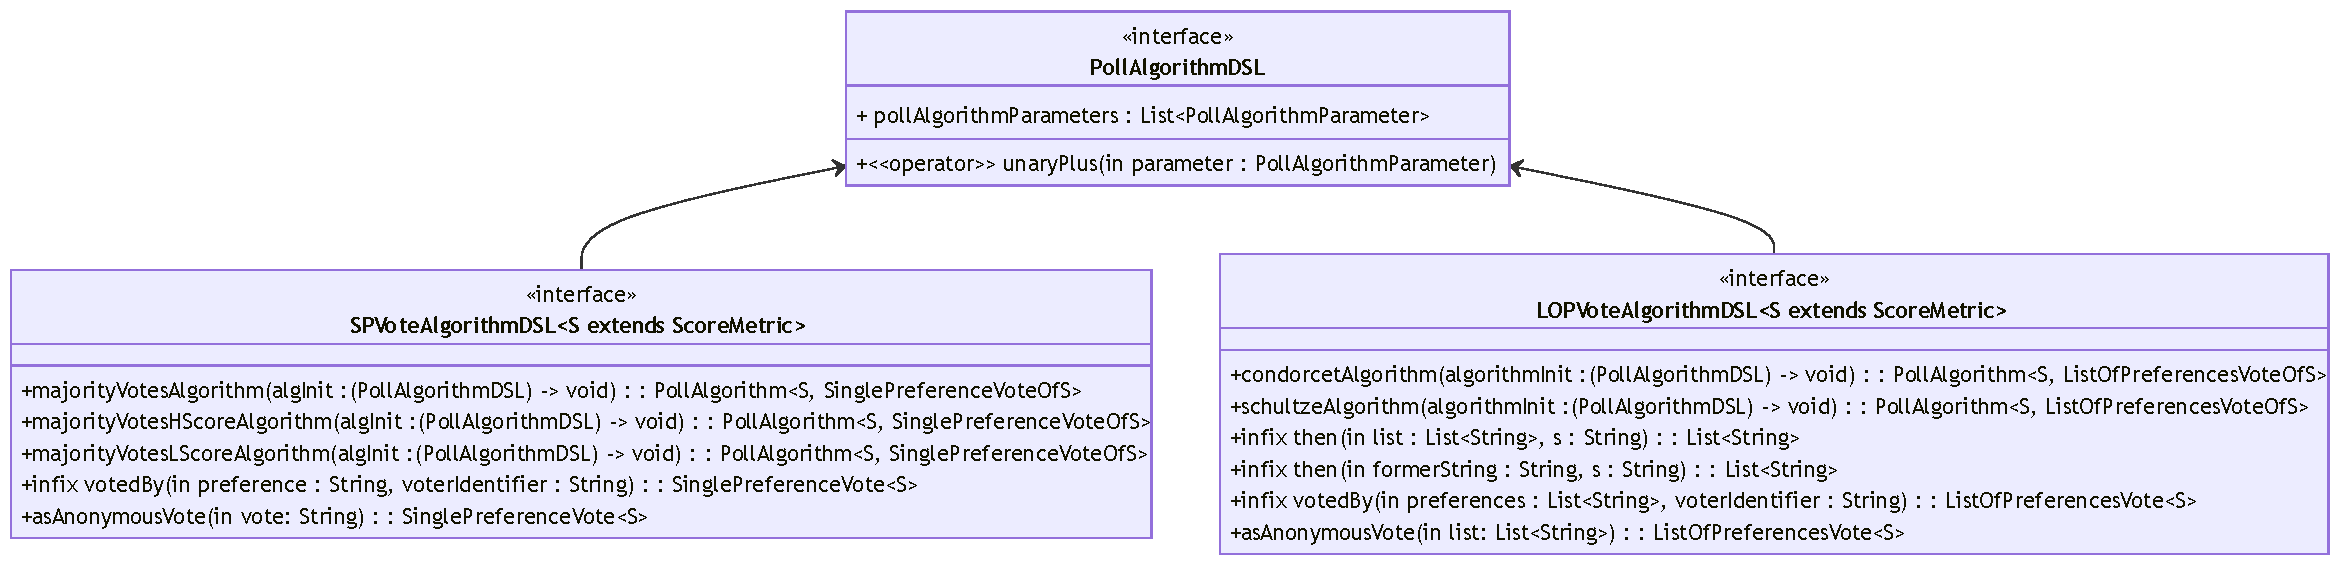
\includegraphics[width=1.1\linewidth]{figures/pollAlgorithmDSL.png}
      \caption{Diagramma UML del \ac{dsl} per la porzione di definizione dell'algoritmo}
     \label{fig:pollAlgorithmDSL}
  \end{figure}
\end{center}
\vfill



\vfill
\begin{center}
 \begin{figure}[H]
     \centering
      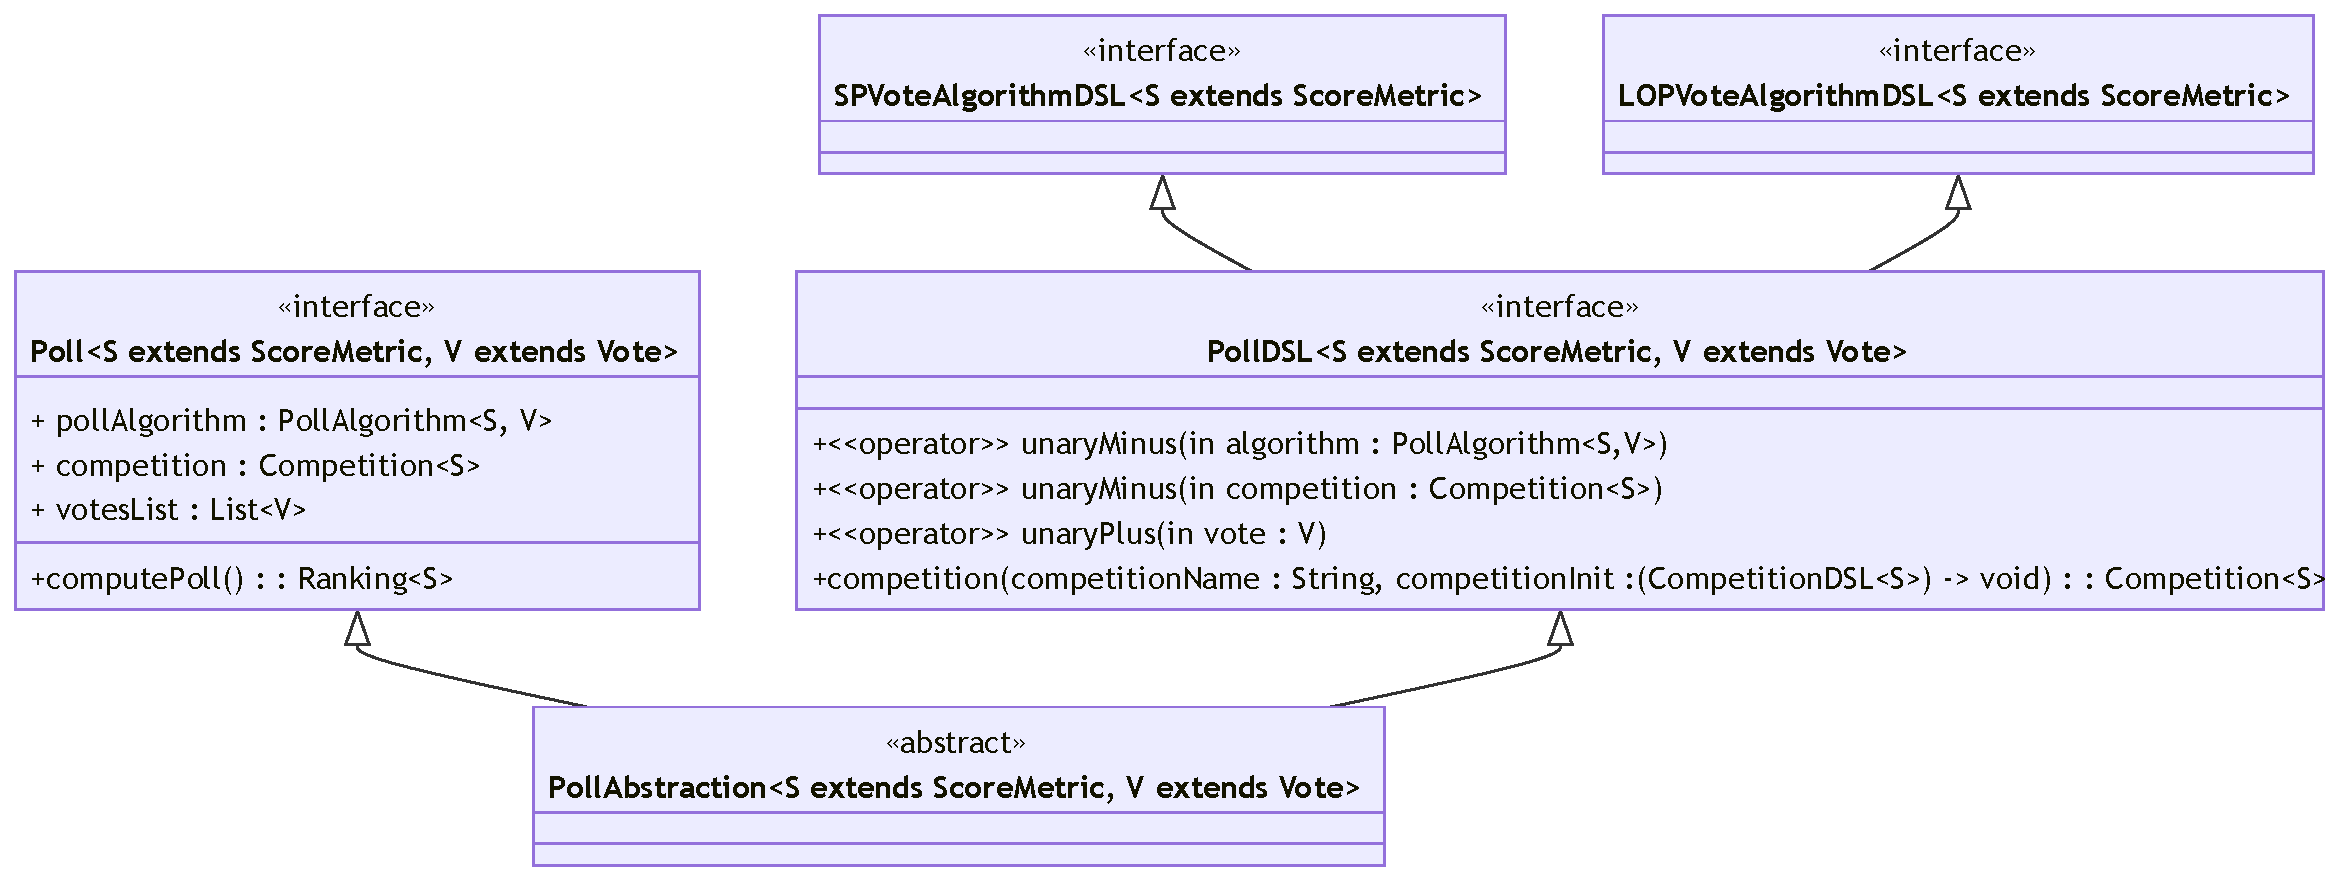
\includegraphics[width=1.1\linewidth]{figures/pollDSL.png}
      \caption{Diagramma UML del \ac{dsl} per la porzione di definizione della votazione}
     \label{fig:pollDSL}
  \end{figure}
\end{center}
\vfill
  



\section{Domain Specific Language per la definizione della competizione}
\label{dslcompetizione}
Questo DSL è pensato per facilitare la creazione ed il popolamento di una competizione.
La funzione \texttt{competitor}, utile alla creazione del concorrente,
richiede che venga definito l'identificativo del concorrente e un inizializzatore in cui saranno definiti i punteggi realizzati.
Il concorrente istanziato, viene aggiunto alla lista dei concorrenti grazie all'uso dell'operatore unario \texttt{+}.

In figura \ref{fig:competitionDSL} viene mostrato il diagramma UML delle interfacce e della classe astratta.
\begin{figure}[H]
    \centering
     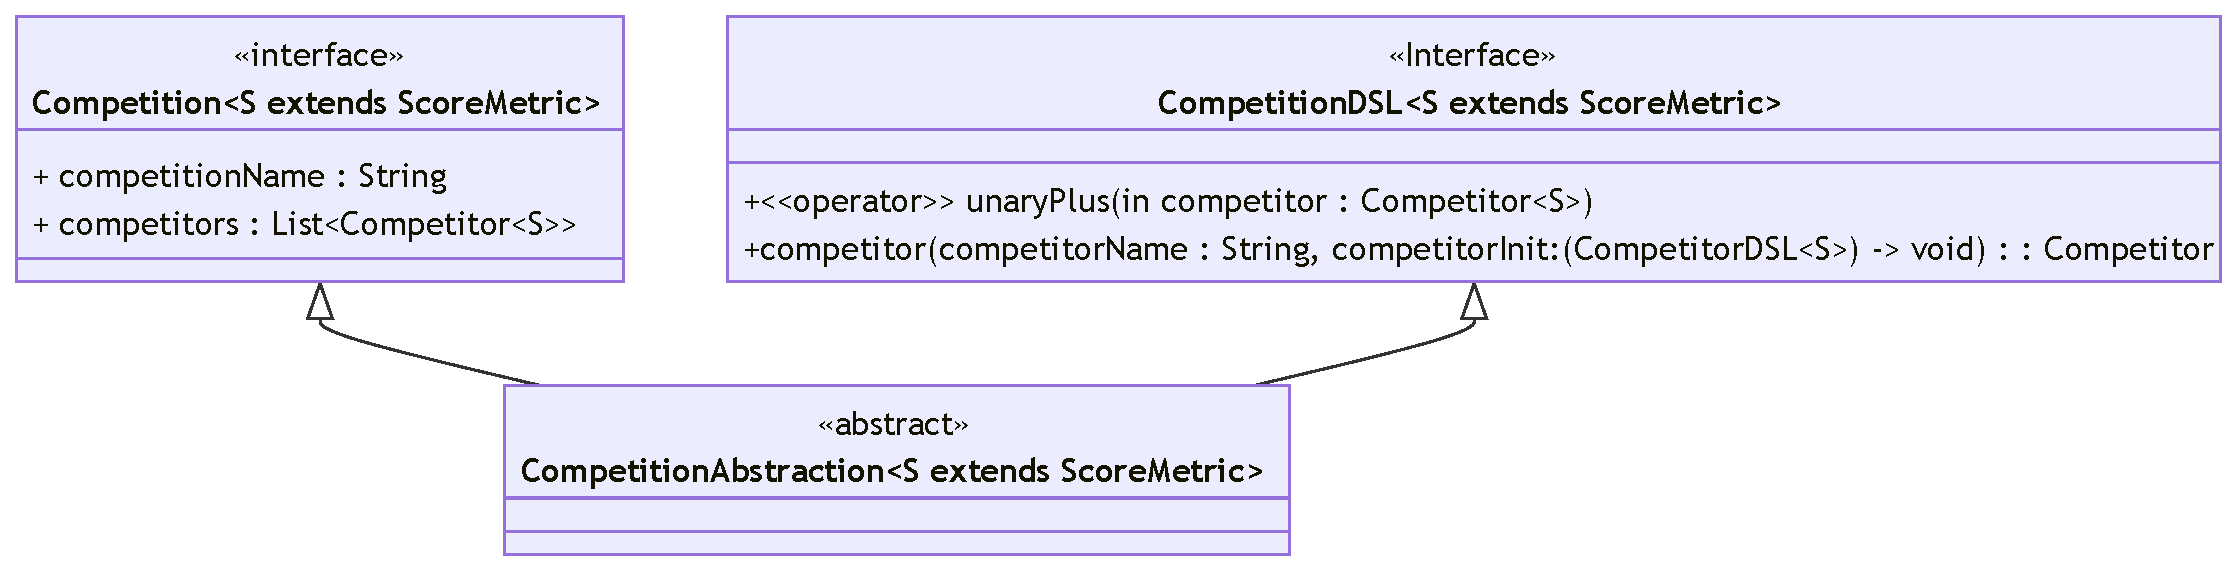
\includegraphics[width=1.1\linewidth]{figures/competitionDSL.png}
     \caption{Diagramma UML del \ac{dsl} per la definizione della competizione}
    \label{fig:competitionDSL}
 \end{figure}
 \newpage
\section{\ac{dsl} per la definizione del concorrente}
Questo DSL è ideato per facilitare la creazione di un concorrente.
Ciascun concorrente può avere un elenco di punteggi, e ciascuno di essi può essere
assegnato al concorrente (vedi capitolo \ref{dslcompetizione} ) attraverso l'uso dell'operatore unario \texttt{+}. .
\begin{figure}[H]
    \centering
     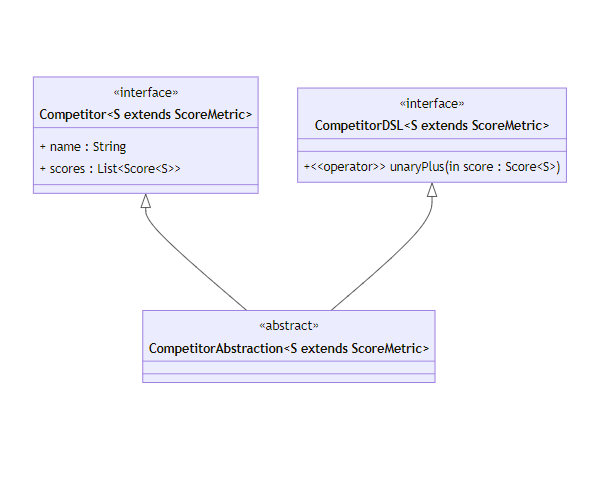
\includegraphics[width=1.1\linewidth]{figures/competitorDSL.png}
     \caption{Diagramma UML del \ac{dsl} per la definizione della concorrente}
    \label{fig:competitorDSL}
 \end{figure}
 \newpage

%----------------------------------------------------------------------------------------
\chapter{Implementazione}

\section{Build automation e versionamento degli artefatti}
L'adozione di un sistema di build automation è un fattore chiave per la produzione
efficace ed efficiente di software di qualità.

Come principio base, è importante che ciascuna modifica apportata al codice
sia testata a livello unitario e abbia documentazione correlata, che sia l'aggiunta 
di una funzionalità piuttosto che la variazione di un campo, a titolo meramente
esemplificativo. 

Inoltre, queste modifiche devono essere ulteriormente 
verificate attraverso test di integrazione, in modo da garantire la piena
compatibilità tra i componenti. 

Le verifiche possono essere effettuate 
manualmente dallo sviluppatore, ma per ridurre il rischio di errori è
possibile adottare un sistema di automazione, che attraverso una serie di task predefiniti
e ripetibili, verifichi automaticamente le varie fasi,
gestendo anche le dipendenze tra i task stessi.
Così facendo, si può subito notare se tutto è andato a buon fine oppure 
se è necessario effettuare ulteriori eventi correttivi.

Una volta che il flusso di compilazione e verifica viene terminato con successo,
è possibile procedere alla generazione di uno o più artefatti e della relativa documentazione.
Questi prodotti possono essere sottoposti ad un operazione di versionamento,
in modo da distinguere le evoluzioni del software e semplificarne la distribuzione
e la tracciabilità.

In questo progetto sono stati adottati \texttt{Kotlin} come linguaggio di programmazione
e \texttt{Gradle} come build automator.

Poichè gli artefatti che vengono generati sono dipendenti dall'architettura della macchina
e dal sistema operativo sui quali avviene il processo di build, è opportuno eseguire tale processo
su piattorme dedicate come Github.
Github fornisce ambienti standard e personalizzabili
in base a direttive, gestendo il processo di \ac{ci}/\ac{cd} che è stato descritto in questo capitolo. 
Infine, per favorire la distribuzione e la compatibilità verso molteplici sistemi,
è utile adottare strumenti come \texttt{Kotlin Multiplatform},
che semplificano la generazione dell'output finale adattandolo alle specifiche piattaforme. 


\subsection{Kotlin Multiplatform}
Kotlin Multiplatform è un tool che favorisce il riuso di codice tra molteplici piattaforme.
Grazie ad esso, riutilizzando la logica applicativa scritta in \textit{Kotlin}, è possibile produrre artefatti compatibili
in molteplici piattaforme, dette anche \textit{target}, come \texttt{JVM}, \texttt{JS}, \texttt{Android}, \texttt{iOS} e piattaforme native come \texttt{Linux}.
I \textit{target} sono disposti secondo una gerarchia predefinita, comunque modificabile in caso di necessità, e sono previsti \textit{target} intermedi.
Per ogni \textit{target} viene definito un \textit{source set}, ossia un insieme di file sorgente, che definisce anche le dipendenze e le compatibilità.
Il \textit{source set} predefinito è \texttt{commonMain}, e contiene il codice comune a tutti i \textit{target}.
Al suo interno è possibile utilizzare funzioni e dipendenze che siano compilabili verso tutte le piattaforme dichiarate, mentre quelle che
sono legate ad uno specifico linguaggio o architettura vanno definite ed utilizzate all'interno degli opportuni \textit{source sets},
come \texttt{jvmMain} e \texttt{jsMain}. 
Un esempio è visibile in figura \ref{fig:targets}, in cui i \textit{target} intermedi sono colorati in azzurro: \textit{apple} conterrà
codice compatibile solamente con i \textit{target} che lo estendono, oltre a quello ereditato dai livelli superiori. Pertanto, è ammesso 
che \textit{macos} utilizzi funzioni che non siano disponibili in \textit{tvos} ma entrambi accedono al codice messo a disposizione da \textit{apple}.

\begin{figure}[H]
    \centering
     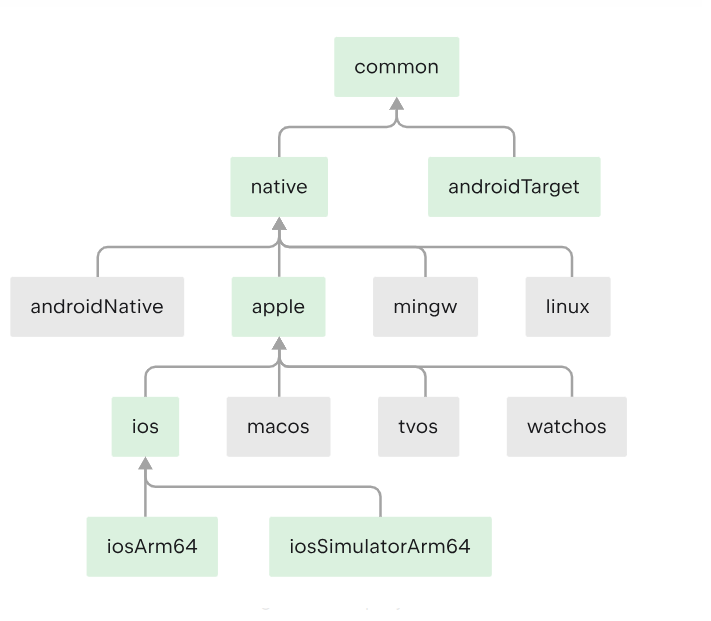
\includegraphics[width=1\linewidth]{figures/mptargets.png}
     \caption{Esempio di una possibile gerarchia di \textit{target}. Fonte: \cite{WebsiteKotlinMultiPlatformTargets}}
    \label{fig:targets}
 \end{figure}

Inoltre, questo meccanismo permette di applicare un \textit{template method} architetturale, grazie al quale è possibile dichiarare nel \textit{
    source set
} \texttt{commonMain} funzioni agnostiche 
tramite la direttiva \texttt{expected}, senza definirne il contenuto, che sarà valorizzato in un successivo momento.
In fase di compilazione, nelle versioni platform-specific, saranno valorizzate tramite funzioni che adottano la direttiva \texttt{actual},
che posso richiamare funzionalità altrimenti non adottabili in \textit{commonMain}.

Una logica analoga è applicabile anche alla sezione dei test: è disponibile un \textit{source set} di base, detto \textit{commonTest}, e altri
eventuali che contengono codice compatibile solo in quella determinata piattaforma.
In figura \ref{fig:sourcesetscompilation} viene mostrato il flusso e gli output ottenuti utilizzando i \textit{target} \texttt{JVM} e \texttt{JS}.

\begin{figure}[H]
    \centering
     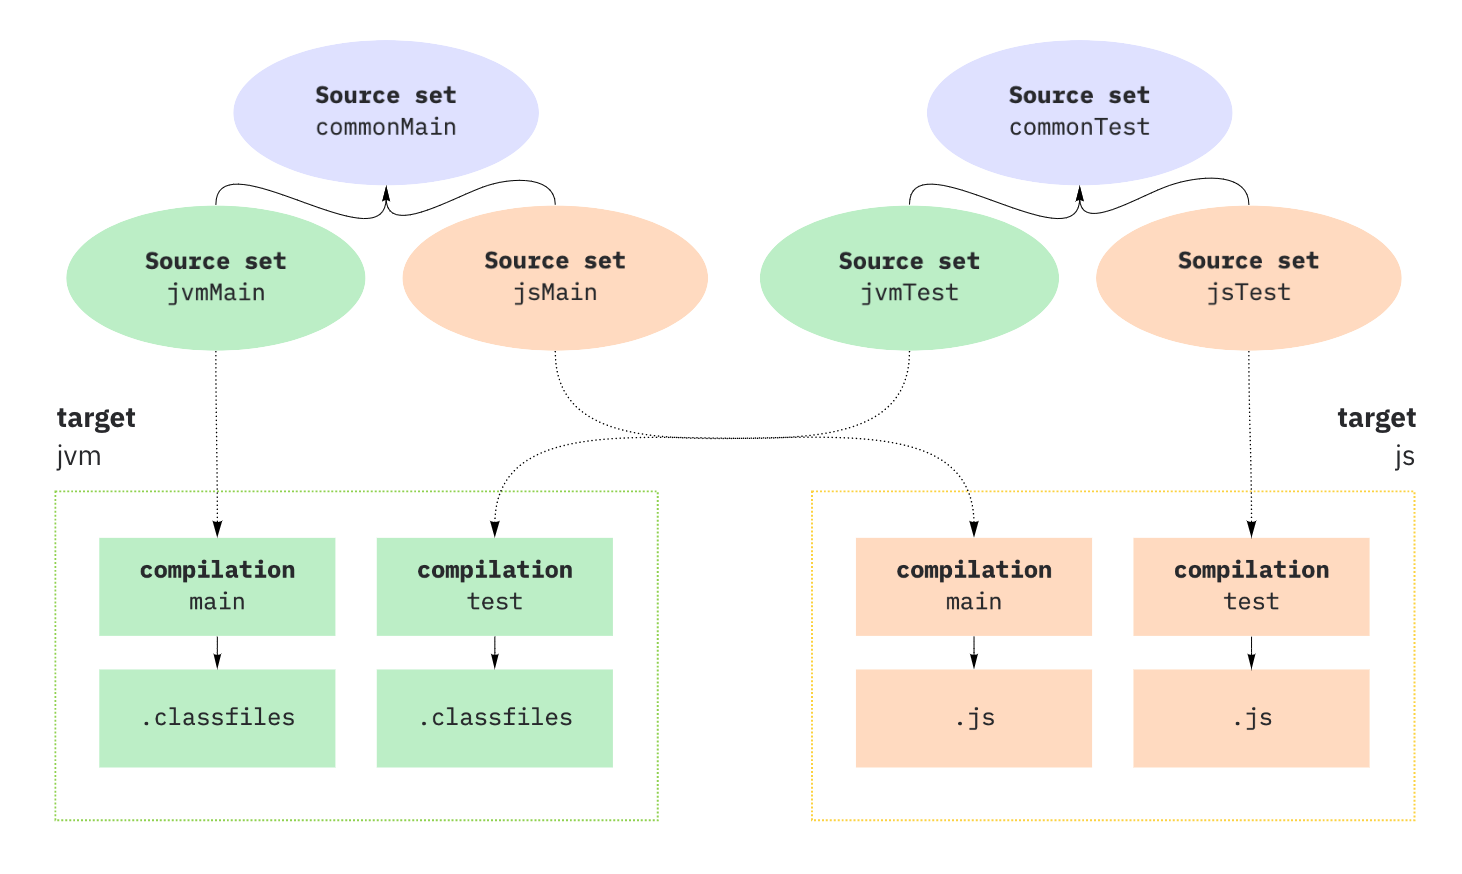
\includegraphics[width=1\linewidth]{figures/sourcesetscompilation.png}
     \caption{Esempio di output ottenibili in un progetto multipiattaforma. Fonte: \cite{WebsiteKotlinMultiPlatformCompilations}}
    \label{fig:targets}
 \end{figure}

\subsection{GitHub Actions}
 \ac{gha} è una piattaforma di \ac{ci}/\ac{cd} basata su repository \ac{gh},
 ai quali possono essere agganciati degli elementi detti workflow.

 Un \texttt{workflow}, definibile attraverso la sintassi \texttt{YAML}, rappresenta una sequenza di azioni che possono essere eseguite
 all'occorrenza di un evento, ad esempio la creazione di un \texttt{tag} nel repository,
 una \texttt{richiesta pull}, un'esecuzione manuale richiesta dal proprietario del repository, ecc\dots

In ogni \texttt{workflow} va specificato il nome dello stesso e l'insieme di eventi che ne scatena 
l'esecuzione. 
Di seguito a ciò, è possibile definire un insieme di \texttt{job}.

Ciascun \texttt{job} è legato ad uno specifico ambiente di esecuzione: va definito che tipo di
sistema operativo deve essere adottato (\texttt{Linux}, \texttt{Windows}, \texttt{macOS})
e se al termine dello stesso debba essere restituito un output, che sarà accessibile da altri \texttt{job}.
È possibile specificare delle variabili in una \texttt{matrice}, in modo eseguire parallelamente molteplici istanze di uno stesso \texttt{job} 
in base alle combinazioni delle variabili; a titolo esemplificativo, eseguire la compilazione di codice utilizzando
la stessa versione del compilatore ma su 3 sistemi operativi differenti.  

Ciascun \texttt{job} è caratterizzato da un proprio flusso indipendente, di conseguenza
per orchestare l'intero processo è opportuno specificare condizioni basate sulle variabili di output 
oppure sull'indicazione del completamento di uno o più i \texttt{jobs} desiderati.

All'interno del \texttt{job} sono definibili uno o più \texttt{step}: questi vengono eseguiti in maniera sequenziale
e sono impostabili per eseguire una sequenza arbitraria di comandi \texttt{bash} oppure
per eseguire una \texttt{action} pubblica.
Quest'ultima rappresenta un ottimo modo di favorire il riuso
e la condivisione di codice nella community \ac{gh}, in quanto è possibile, ad esempio, utilizzare un workflow complesso
come se fosse un singolo step (\texttt{composite action}) oppure lanciare l'esecuzione di un container senza
imporre \textit{effort} riguardo alla gestione delle dipendenze e delle configurazioni (\texttt{docker container action}).

\subsection{GitHub Pages}
 \ac{ghp} è un servizio di hosting disponibile per ogni account ed organizzazione in \ac{gh},
 attraverso il quale è possibile pubblicare un sito web statico, che viene costruito e
 pubblica attraverso un apposito \texttt{workflow} predefinito. 
 Nel caso di un iniziativa progettuale come una libreria, può essere utilizzato dare informazioni 
 su come scaricare ed installare il software oppure per pubblicare la documentazione.

\subsection{Maven Central, GitHub Packages e NPM}
Maven Central è tra i repository centralizzati più popolari per distribuire e riutilizzare artefatti basati su \ac{jvm}.
Un repository è definibile come "la directory che memorizza tutti i progetti e le librerie JAR, i plugin
o qualsiasi altro artefatto specifico del progetto che può essere facilmente utilizzato da Maven"\cite{kozak2022three}.

Il sistema di gestione delle dipendenze di Maven è in grado di risolvere automaticamente le dipendenze transitive,
semplificando la gestione manuale delle dipendenze per gli sviluppatori. 
Gli artefatti caricati su Maven Central, tra cui librerie di codice compilato, documentazione ed elenco di dipendenze,
sono immutabili e non possono essere modificati né eliminati.
Le dipendenze vengono identificate in modo univoco con una tripletta \texttt{groupId:artifactId:version},
dove \texttt{groupId} identifica un gruppo di artefatti, \texttt{artifactId} si riferisce al nome della libreria
e \texttt{version} identifica univocamente ogni rilascio della libreria.
Ad esempio, la tripletta 'org.jetbrains.kotlinx:kotlinx-serialization-json:1.6.0' 
identifica la versione 1.6.0 di un serializzatore json per \textit{Kotlin}, gestito da \textit{JetBrains}.

Tutte le versioni di una libreria rilasciate su Maven Central, una volta pubblicate sono sempre disponibili nel repository. 
Gli utenti della libreria sono liberi di decidere quale versione utilizzare e per quanto tempo e a questi ultimi è delegata la responsabilità di aggiornare le proprie dipendenze per 
adeguarsi a problemi di sicurezza o evoluzioni dell'API.
Nel lungo termine, queste decisioni determinano le librerie e le versioni più popolari nell'intero ecosistema software.
Si osserva che per la maggior parte delle librerie, più di una versione è attivamente utilizzata in un dato momento \cite{soto2019emergence}. 

Dallo studio empirico condotto da \cite{soto2019emergence}, è emerso che "circa il 40\% delle librerie ha due o più versioni attivamente utilizzate, 
mentre quasi il 4\% non ha mai avuto alcun utente su Maven Central. 
Inoltre, si è scoperto che più del 90\% delle versioni più popolari non sono le ultime versioni rilasciate, 
e sia le versioni attive che significativamente popolari sono distribuite lungo la storia delle versioni della libreria".

Un' alternativa all'uso di Maven Central può risiedere in \ac{gh} Packages. Quest'ultimo pone una gestione 
semplificata per la pubblicazione degli artefatti, in quanto strettamente connesso all'uso di repository \ac{gh},
il che permette di avere un controllo degli accessi efficace come quello disponibile per i repo.
Al pari di Maven Central viene mantenuto il concetto di artefatti immutabili, e in più viene dato il supporto
per l'archiviazione di pacchetti in numerosi linguaggi, tra cui \textit{C\#}.

Un altro famoso gestore di pacchetti è \ac{npm}, focalizzato sulle diffusione di librerie \textit{Javascript} e \textit{Node.js},
si differenzia in particolare dai precedenti in quanto non adotta il principio di immutabilità.
In questo caso, la modifica o eliminazione di una versione di un pacchetto può avere impatti notevoli sugli utilizzatori,
portando a potenziali disastri mondiali \cite{NPMChaos}.

\section{DSL }
come ho utilizzato gli operator le lambda with receiver esempi di utilizzo del dsl
tanti esempi nei listings

\section{Librerie multiplatform utilizzate}

\section{Pubblicazione di artefatti}
Spiegare brevemente i passaggi necessari che sono stati fatti per arrivare
alle pubblicazioni

\section{Pubblicazione della documentazione}
spiegare la creazione di un nuovo workflow, e collegato a quelli esistenti
%----------------------------------------------------------------------------------------
\chapter{Valutazione}

\section{Test realizzati}
Descrivere le varie situazioni che sono andato a controllare,
mettendo dettagli solo per i casi più complicati

\section{Sperimentazione con Ergast API}
La sperimentazione della libreria \texttt{EleKtion} è stata effettuata applicando ad essa un
caso di studio reale, nello specifico applicando gli algoritmi di votazione ai risultati 
delle gare di \textit{\ac{f1}}.

I dati sono accessibili attraverso un API REST pubblica chiamata Ergast API \cite{WebsiteErgastAPI},
disponibile per scopi non-commerciali,
che mette a disposizione dati inerenti ai mondiali di \textit{\ac{f1}} a partire dal primo (1950).
Per ognuno di questi sono a disposizione numerose informazioni come l'elenco delle gare (Gran Premi),
e per ognuna di esse le gare di qualifica, le classifiche generali dei piloti, i risultati delle gare ufficiali, lo storico
dei piloti, le classifiche generali dei costruttori e molto altro.

Allo scopo di questa tesi, sono risultate utili le informazioni riguardo ai risultati delle gare ufficiali (legate ad uno specifico anno)
e le classifiche generali (legate ad uno specifico anno) al termine di ogni gara.

Attaverso appositi endpoint, è stato possibile scaricare i dati necessari per predisporre le informazioni necessarie
ad \texttt{EleKtion}, utilizzando come voti gli esiti delle varie gare, e applicando gli algoritmi a lista di preferenze.
L'elemento più favorito nel voto è rappresentato dal pilota che si è classificato primo in gara, mentre l'elemento più sfavorito
è stato cosiderato il pilota classificatosi in gara.

Nei seguenti sottocapitoli vengono mostrati i passaggi effettuati per elaborare i dati di un mondiale,
in particolare vengono generate come output delle votazioni le classifiche parziali al termine di ogni gara in modo da avere uno storico,
che verrà confrontato con lo storico delle classifiche reali.
Verrà infine svolto un calcolo utile ad indicare
la differenza in termini qualitativi tra i dati generati dalle votazioni con differenti algoritmi 
e quelli ottenuti al termine della votazione.

\subsection{Elaborazione dati di un mondiale \textit{F1}}
\label{chapter:elaborazionemondiale}
Si è provveduto ad ottenere l'elenco delle gare svoltesi nel corso del mondiale AAAA (anno del mondiale), disponibili
al seguente indirizzo \texttt{https://ergast.com/api/f1/AAAA.json}.

In questo mondiale sono state effettuate in totale \textit{k} gare, per ognuna di esse sono stati scaricati i
dati di gara, tenendo in considerazione solamente il nominativo del pilota e la posizione di arrivo.
Eventuali ritiri a causa di guasti o altri motivi non sono trattati, facendo fede alla posizione restituita dall'API.

Al termine si ha quindi una \texttt{Map<String, List<Pair<String, Int>>>}, nella quale le chiavi sono rappresentate 
dal nome della gara (es. Australian-Grand-Prix-1-2008, Malaysian-Grand-Prix-2-2008, ecc...) i valori liste in cui per
ogni elemento contiene una tupla rappresentata dal nominativo del pilota e la posizione di arrivo.

Come visibile nell'estratto di codice \ref{lst:election-GPs}, si organizzano tante votazioni indipendenti quante sono le
gare presenti nel mondiale:
Viene definito l'elenco complessivo dei nominativi presenti nelle varie gare, in modo da
avere un censimento di tutti i possibili candidati. Per la prima votazione vengono definiti tutti i candidati ammissibili,
che per motivi di funzionamento dell'algoritmo, vengono passati anche coloro che effettivamente non sono presenti in quella gara
ma in altre sì (ad esempio infortuni, sostituzioni, ecc...). Si definisce l'algoritmo da utilizzare, in questo caso sono
ammissibili l'algoritmo di Condorcet o l'algoritmo di Schultze. 
Succesivamente si definisce l'elenco di voti, che consiste in un unico voto
identificabile nell'elenco dei nominativi dei piloti secondo l'ordine di arrivo reale (dal primo all'ultimo), e come votante si può definire il nome del circuito
di gara. Se un pilota è assente in quella gara ma presente in altre, tramite l'elenco dei possibili candidati
vengono definiti chi sono in questa situazione e vengono "virtualmente" posti ad ultimi in modo da avere la lunghezza della lista 
di preferenze uniforme al numero dei possibili candidati.
Infine, questa votazione viene inserita nell'elenco delle votazioni da elaborare.

Per la seconda votazione viene considerata anche la seconda gara, e mantenendo stabile l'insieme dei possibili candidati e l'algoritmo da usare,
vengono considerati come voti l'elenco dei nominativi dei piloti (secondo l'ordine di arrivo reale) della prima gara
e l'elenco dei nominativi dei piloti (secondo l'ordine di arrivo reale) della seconda gara.
Proseguendo nell'esecuzione, si arriva ad avere \textit{k} votazioni indipendenti, in cui l'ultima conterrà
come voti gli esiti delle varie gare dalla prima all' \textit{k}-esima.

La generazione delle classifiche parziali secondo l'algoritmo selezionato, fornisce una serie di risultati in
cui il primo consiste nella classifica parziale al termine dell'ultima gara, il secondo nella classifica parziale al termine 
della seconda gara, fino ad arrivare alla classifica finale.

I dati delle classifiche reali sono ottenuti contattando l'endpoint \texttt{https://ergast.com/api/f1/AAAA/GP/driverStandings.json}",
dove AAAA è l'anno del mondiale e GP è il numero della gara

\lstinputlisting[float,language=Kotlin,label={lst:election-GPs}, caption={Generazione delle classifiche parziali utilizzando \texttt{EleKtion}}]{listings/election-GPs.kt}

Per confrontare gli esiti ottenuti tra i differenti algoritmi, e tra questi e i dati reali estratti dall'API,
è necessario organizzare i dati secondo una matrice \textit{r x k}, dove ogni riga \textit{r} identifica un pilota,
e ogni colonna \textit{k} identifica una gara (o il suo numero progressivo). Nell'incrocio è presente la
posizione nella classifica parziale (reale o generata) ottenuta dal \textit{r}-esimo pilota al termine della
\textit{k}-esima gara.

Per fare un confronto qualitativo tra matrici è fondamentale organizzarle in modo tale le righe e le colonne
siano ordinate allo stesso modo. Nel caso delle righe è possibile adottare un ordinamento lessicografico o 
l'ordinamento presente in una delle matrici, che viene preso come riferimento per le altre.
Nei casi d'uso realizzati, sono state calcolate per prime le classifiche ottenute applicando l'algoritmo di Condorcet,
poi l'ordine dei piloti nella classifica finale è stato preso come riferimento di ordinamento.
Le classifiche ottenute con l'algoritmo di Schultze è stato organizzato secondo lo stesso riferimento e così anche
la classifiche reali. Si rimanda agli estratti di codice \ref{lst:ordering-rankings-condorcet}, \ref{lst:ordering-rankings-schultze},
\ref{lst:ordering-rankings-real} per approfondire l'implementazione di questi criteri.

Esistono numerose metriche di confronto tra matrici, in questo caso si è optato per la \textit{norma di Frobenius}\cite{golub2013matrix},
rappresentata dalla formula $\sqrt{\sum_{i,j}^{} abs(a_{i,j})^2}$, dove $a$ è una matrice che ricavata dalla
differenza tra le matrici trattate.

\lstinputlisting[language=Kotlin,label={lst:ordering-rankings-condorcet}, caption={Ordinamento propedeutico al confronto (Condorcet)}]{listings/ordering-rankings-Condorcet.kt}
\lstinputlisting[language=Kotlin,label={lst:ordering-rankings-schultze}, caption={Ordinamento propedeutico al confronto (Schultze)}]{listings/ordering-rankings-Schultze.kt}
\lstinputlisting[language=Kotlin,label={lst:ordering-rankings-real},caption={Ordinamento propedeutico al confronto (Dati reali)}]{listings/ordering-rankings-real.kt}

\subsection{Elaborazione del mondiale F1 2023}

Si è provveduto alla generazione delle classifiche parziali e della classifica finale 
seguendo il flusso rappresentato in \label{chapter:elaborazionemondiale}.

Si riporta in tabella \ref{tabella:classificafinale2023} gli ordinamenti ottenuti nelle
classifiche finali usando l'algoritmo di Condorcet, l'algoritmo di Schultze e la classifica finale reale

\begin{table}[H]
    \centering
    \begingroup
\resizebox{\linewidth}{!}{%
    \begin{tabular}{|p|p|p|p|}

    \hline
    \multicolumn{1}{|l|}{Posizione} & \multicolumn{1}{l|}{Reali} & \multicolumn{1}{l|}{Condorcet} & \multicolumn{1}{l|}{Schultze} 
 

\end{tabular}}
    \endgroup

    \caption{Tabella relativa al Mondiale \textit{\ac{f1}} 2023, in cui per ogni gara (G*)  è riportata la posizione del concorrente (C*) in classifica generale, al termine della gara stessa.
    I valori sono ricavati da Ergast API \cite{WebsiteErgastAPIStandings}}
    \label{table:classifichegeneralireali2023}
\end{table}


%%2023
\begin{table}[H]
    \centering
    \begingroup
\resizebox{\linewidth}{!}{%
    \begin{tabular}{|c|c|c|c|c|c|c|c|c|c|c|c|c|c|c|c|c|c|c|c|c|c|c|}

    \hline
    \multicolumn{1}{|l|}{} & \multicolumn{1}{l|}{G1} & \multicolumn{1}{l|}{G2} & \multicolumn{1}{l|}{G3} & \multicolumn{1}{l|}{G4} & \multicolumn{1}{l|}{G5} & \multicolumn{1}{l|}{G6} & \multicolumn{1}{l|}{G7} & \multicolumn{1}{l|}{G8} & \multicolumn{1}{l|}{G9} & \multicolumn{1}{l|}{G10} & \multicolumn{1}{l|}{G11} & \multicolumn{1}{l|}{G12} & \multicolumn{1}{l|}{G13} & \multicolumn{1}{l|}{G14} & \multicolumn{1}{l|}{G15} & \multicolumn{1}{l|}{G16} & \multicolumn{1}{l|}{G17} & \multicolumn{1}{l|}{G18} & \multicolumn{1}{l|}{G19} & \multicolumn{1}{l|}{G20} & \multicolumn{1}{l|}{G21} & \multicolumn{1}{l|}{G22} \\ \hline
    C1. & 1 & 1 & 1 & 1 & 1 & 1 & 1 & 1 & 1 & 1 & 1 & 1 & 1 & 1 & 1 & 1 & 1 & 1 & 1 & 1 & 1 & 1 \\ \hline
    C2. & 2 & 2 & 2 & 2 & 2 & 2 & 2 & 2 & 2 & 2 & 2 & 2 & 2 & 2 & 2 & 2 & 2 & 2 & 2 & 2 & 2 & 2 \\ \hline
    C3. & 5 & 5 & 4 & 4 & 4 & 4 & 4 & 4 & 4 & 4 & 4 & 4 & 4 & 4 & 3 & 3 & 3 & 3 & 3 & 3 & 3 & 3 \\ \hline
    C4. & 3 & 3 & 3 & 3 & 3 & 3 & 3 & 3 & 3 & 3 & 3 & 3 & 3 & 3 & 4 & 4 & 4 & 4 & 5 & 4 & 5 & 4 \\ \hline
    C5. & 4 & 4 & 5 & 5 & 5 & 6 & 6 & 5 & 5 & 5 & 6 & 7 & 5 & 5 & 5 & 5 & 5 & 5 & 4 & 6 & 4 & 7 \\ \hline
    C6. & 19 & 8 & 10 & 6 & 7 & 7 & 7 & 7 & 6 & 7 & 7 & 5 & 6 & 6 & 6 & 6 & 6 & 7 & 7 & 7 & 7 & 5 \\ \hline
    C7. & 17 & 20 & 8 & 9 & 9 & 11 & 11 & 11 & 10 & 9 & 8 & 8 & 8 & 8 & 8 & 7 & 7 & 6 & 6 & 5 & 6 & 6 \\ \hline
    C8. & 7 & 6 & 7 & 7 & 6 & 5 & 5 & 6 & 7 & 6 & 5 & 6 & 7 & 7 & 7 & 8 & 8 & 8 & 8 & 8 & 8 & 8 \\ \hline
    C9. & 6 & 7 & 6 & 8 & 8 & 8 & 8 & 8 & 8 & 8 & 9 & 9 & 9 & 9 & 9 & 10 & 10 & 11 & 11 & 10 & 10 & 10 \\ \hline
    C10. & 20 & 19 & 13 & 11 & 14 & 13 & 13 & 14 & 14 & 11 & 11 & 11 & 12 & 12 & 11 & 9 & 9 & 9 & 9 & 9 & 9 & 9 \\ \hline
    C11. & 9 & 11 & 14 & 14 & 10 & 10 & 10 & 10 & 11 & 12 & 12 & 12 & 10 & 10 & 10 & 11 & 11 & 10 & 10 & 11 & 11 & 11 \\ \hline
    C12. & 10 & 13 & 18 & 17 & 18 & 18 & 18 & 12 & 13 & 13 & 13 & 13 & 13 & 13 & 13 & 13 & 13 & 13 & 13 & 13 & 13 & 13 \\ \hline
    C13. & 18 & 10 & 12 & 13 & 12 & 9 & 9 & 9 & 9 & 10 & 10 & 10 & 11 & 11 & 12 & 12 & 12 & 12 & 12 & 12 & 12 & 12 \\ \hline
    C14. & 11 & 14 & 16 & 16 & 16 & 16 & 16 & 17 & 17 & 17 & 17 & 17 & 17 & 17 & 17 & 17 & 17 & 16 & 16 & 14 & 14 & 14 \\ \hline
    C15. & 8 & 9 & 11 & 12 & 13 & 14 & 14 & 15 & 15 & 15 & 15 & 15 & 15 & 15 & 15 & 15 & 14 & 14 & 14 & 15 & 15 & 15 \\ \hline
    C16. & 15 & 15 & 9 & 10 & 11 & 12 & 12 & 13 & 12 & 14 & 14 & 14 & 14 & 14 & 14 & 14 & 15 & 15 & 15 & 16 & 16 & 16 \\ \hline
    C17. & 16 & 17 & 15 & 15 & 15 & 15 & 15 & 16 & 16 & 16 & 16 & 16 & 16 & 16 & 16 & 16 & 16 & 17 & 18 & 18 & 18 & 18 \\ \hline
    C18. & 13 & 12 & 17 & 18 & 17 & 17 & 17 & 18 & 18 & 18 & 18 & 18 & 18 & 18 & 18 & 18 & 18 & 18 & 19 & 19 & 19 & 19 \\ \hline
    C19. & 12 & 16 & 19 & 19 & 19 & 20 & 20 & 20 & 19 & 19 & 19 & 19 & 19 & 19 & 20 & 20 & 20 & 20 & 21 & 21 & 21 & 21 \\ \hline
    C20. & 14 & 18 & 20 & 20 & 20 & 19 & 19 & 19 & 20 & 20 & 20 & 20 & 20 & 21 & 21 & 21 & 21 & 21 & 22 & 22 & 22 & 22 \\ \hline
    C21. & 20 & 20 & 20 & 20 & 20 & 20 & 20 & 20 & 20 & 20 & 21 & 21 & 21 & 22 & 22 & 22 & 22 & 22 & 17 & 17 & 17 & 17 \\ \hline
    C22. & 20 & 20 & 20 & 20 & 20 & 20 & 20 & 20 & 20 & 20 & 21 & 21 & 22 & 20 & 19 & 19 & 19 & 19 & 20 & 20 & 20 & 20 \\ \hline
    \end{tabular}}
    \endgroup

    \caption{Tabella relativa al Mondiale \textit{\ac{f1}} 2023, in cui per ogni gara (G*)  è riportata la posizione del concorrente (C*) in classifica generale, al termine della gara stessa.
    I valori sono ricavati da Ergast API \cite{WebsiteErgastAPIStandings}}
    \label{table:classifichegeneralireali2023}
\end{table}

\begin{figure}[H]
    \centering
     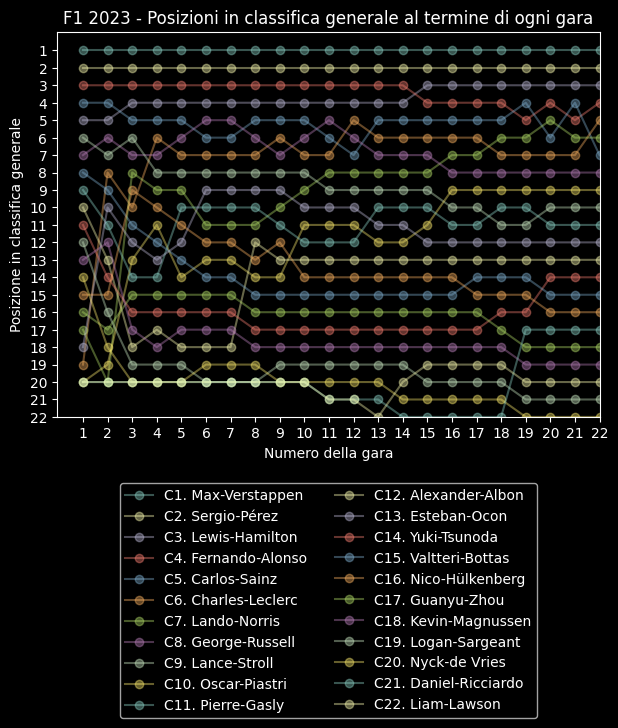
\includegraphics[scale=1.0]{figures/realstandings2023.png}
     \caption{Rappresentazione grafica della tabella \ref{table:classifichegeneralireali} }
 \end{figure}


 \begin{table}[H]
    \centering
    \begingroup
    \resizebox{\linewidth}{!}{%
    \begin{tabular}{|c|c|c|c|c|c|c|c|c|c|c|c|c|c|c|c|c|c|c|c|c|c|c|}

    \hline
    \multicolumn{1}{|l|}{} & \multicolumn{1}{l|}{G1} & \multicolumn{1}{l|}{G2} & \multicolumn{1}{l|}{G3} & \multicolumn{1}{l|}{G4} & \multicolumn{1}{l|}{G5} & \multicolumn{1}{l|}{G6} & \multicolumn{1}{l|}{G7} & \multicolumn{1}{l|}{G8} & \multicolumn{1}{l|}{G9} & \multicolumn{1}{l|}{G10} & \multicolumn{1}{l|}{G11} & \multicolumn{1}{l|}{G12} & \multicolumn{1}{l|}{G13} & \multicolumn{1}{l|}{G14} & \multicolumn{1}{l|}{G15} & \multicolumn{1}{l|}{G16} & \multicolumn{1}{l|}{G17} & \multicolumn{1}{l|}{G18} & \multicolumn{1}{l|}{G19} & \multicolumn{1}{l|}{G20} & \multicolumn{1}{l|}{G21} & \multicolumn{1}{l|}{G22} \\ \hline
    C1. & 1 & 1 & 1 & 1 & 1 & 1 & 1 & 1 & 1 & 1 & 1 & 1 & 1 & 1 & 1 & 1 & 1 & 1 & 1 & 1 & 1 & 1 \\ \hline
    C2. & 2 & 1 & 2 & 1 & 2 & 2 & 2 & 2 & 2 & 2 & 2 & 2 & 2 & 2 & 2 & 2 & 2 & 2 & 2 & 2 & 2 & 2 \\ \hline
    C3. & 5 & 3 & 4 & 3 & 5 & 4 & 4 & 3 & 4 & 3 & 4 & 4 & 4 & 4 & 4 & 3 & 4 & 4 & 4 & 3 & 4 & 3 \\ \hline
    C4. & 3 & 2 & 3 & 2 & 3 & 3 & 3 & 2 & 3 & 2 & 3 & 3 & 3 & 3 & 3 & 3 & 3 & 3 & 3 & 3 & 3 & 4 \\ \hline
    C5.  & 4 & 3 & 5 & 3 & 4 & 5 & 6 & 4 & 5 & 5 & 7 & 7 & 7 & 6 & 5 & 4 & 5 & 5 & 5 & 4 & 5 & 4 \\ \hline
    C6.  & 19 & 10 & 14 & 11 & 6 & 7 & 7 & 6 & 7 & 5 & 6 & 6 & 6 & 6 & 7 & 5 & 5 & 7 & 5 & 6 & 5 & 4 \\ \hline
    C7. & 17 & 11 & 13 & 7 & 11 & 10 & 11 & 10 & 11 & 8 & 10 & 9 & 8 & 7 & 8 & 6 & 6 & 6 & 6 & 5 & 6 & 5 \\ \hline
    C8. & 7 & 4 & 7 & 4 & 6 & 6 & 5 & 5 & 6 & 4 & 5 & 5 & 5 & 5 & 6 & 5 & 7 & 6 & 7 & 5 & 7 & 6 \\ \hline
    C9. & 6 & 11 & 6 & 4 & 6 & 9 & 7 & 7 & 8 & 6 & 8 & 8 & 8 & 7 & 9 & 9 & 9 & 10 & 9 & 9 & 8 & 7 \\ \hline
    C10.  & 20 & 11 & 14 & 8 & 15 & 12 & 12 & 10 & 13 & 10 & 11 & 12 & 9 & 10 & 11 & 8 & 8 & 9 & 8 & 8 & 9 & 7 \\ \hline
    C11. & 9 & 5 & 8 & 6 & 7 & 8 & 8 & 8 & 9 & 7 & 9 & 10 & 8 & 8 & 10 & 7 & 8 & 8 & 8 & 7 & 8 & 8 \\ \hline
    C12.  & 10 & 11 & 14 & 11 & 13 & 13 & 16 & 12 & 14 & 11 & 11 & 13 & 9 & 9 & 11 & 8 & 9 & 10 & 9 & 9 & 10 & 9 \\ \hline
    C13.  & 18 & 10 & 11 & 9 & 9 & 9 & 9 & 8 & 10 & 9 & 11 & 11 & 9 & 9 & 11 & 9 & 9 & 11 & 9 & 10 & 11 & 9 \\ \hline
    C14.  & 11 & 6 & 8 & 5 & 8 & 9 & 10 & 9 & 12 & 12 & 13 & 13 & 11 & 12 & 13 & 11 & 11 & 13 & 11 & 11 & 13 & 10 \\ \hline
    C15.  & 8 & 10 & 11 & 9 & 12 & 11 & 13 & 11 & 13 & 11 & 12 & 13 & 10 & 11 & 12 & 10 & 10 & 12 & 10 & 12 & 12 & 11 \\ \hline
    C16. & 15 & 8 & 9 & 7 & 10 & 11 & 11 & 12 & 15 & 13 & 14 & 14 & 12 & 13 & 14 & 12 & 12 & 14 & 12 & 12 & 14 & 11 \\ \hline
    C17.  & 16 & 9 & 10 & 10 & 13 & 12 & 14 & 13 & 15 & 13 & 15 & 14 & 13 & 14 & 15 & 13 & 13 & 15 & 13 & 13 & 15 & 12 \\ \hline
    C18. & 13 & 7 & 12 & 9 & 9 & 12 & 13 & 13 & 15 & 15 & 16 & 15 & 14 & 15 & 16 & 14 & 14 & 16 & 14 & 14 & 16 & 13 \\ \hline
    C19.  & 12 & 10 & 13 & 11 & 16 & 14 & 17 & 15 & 17 & 15 & 18 & 16 & 15 & 16 & 17 & 15 & 15 & 17 & 15 & 15 & 17 & 14 \\ \hline
    C20.  & 14 & 9 & 12 & 11 & 14 & 13 & 15 & 14 & 16 & 14 & 17 & 16 & 16 & 17 & 18 & 16 & 16 & 18 & 16 & 16 & 18 & 15 \\ \hline
    C21. & 21 & 12 & 15 & 12 & 17 & 15 & 18 & 16 & 18 & 16 & 19 & 17 & 17 & 18 & 19 & 17 & 17 & 19 & 17 & 17 & 19 & 16 \\ \hline
    C22.  & 22 & 13 & 16 & 13 & 18 & 16 & 19 & 17 & 19 & 17 & 20 & 18 & 18 & 19 & 20 & 18 & 18 & 20 & 18 & 18 & 20 & 17 \\ \hline
    \end{tabular}}
    \endgroup

    \caption{Tabella relativa al Mondiale \textit{\ac{f1}} 2023, in cui per ogni gara (G*)  è riportata la posizione del concorrente (C*) in classifica generale, al termine della gara stessa.
    I valori sono ricavati dall'applicazione dell'algoritmo di Condorcet al termine di ogni gara, considerando anche le precedenti.
    Ogni gara rappresenta un voto, composto dagli ordini di arrivo.
    }
    \label{table:classifichegeneralicondorcet2023}
\end{table}

\begin{figure}[H]
    \centering
     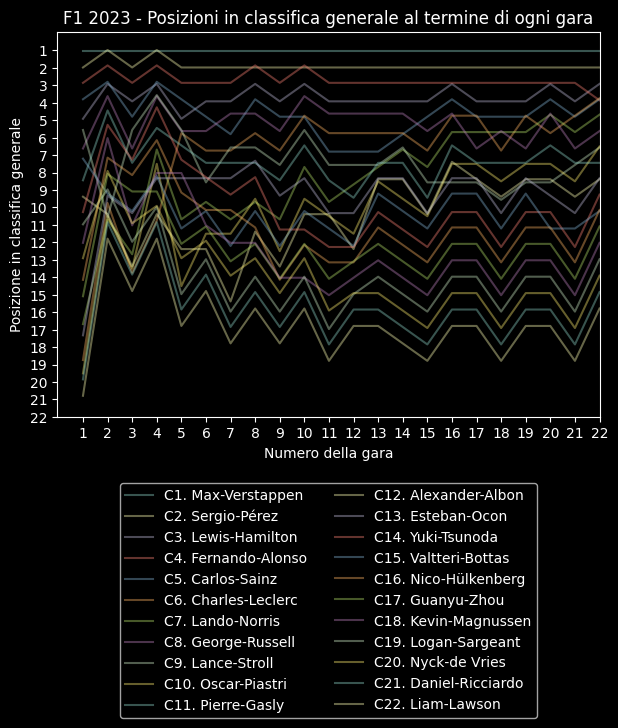
\includegraphics[scale=1.0]{figures/condorcetstandings2023.png}
     \caption{Rappresentazione grafica della tabella \ref{table:classifichegeneralicondorcet} }
 \end{figure}


 \begin{table}[H]
    \centering
    \begingroup
    \resizebox{\linewidth}{!}{%
    \begin{tabular}{|c|c|c|c|c|c|c|c|c|c|c|c|c|c|c|c|c|c|c|c|c|c|c|}
  
    \hline
    \multicolumn{1}{|l|}{} & \multicolumn{1}{l|}{G1} & \multicolumn{1}{l|}{G2} & \multicolumn{1}{l|}{G3} & \multicolumn{1}{l|}{G4} & \multicolumn{1}{l|}{G5} & \multicolumn{1}{l|}{G6} & \multicolumn{1}{l|}{G7} & \multicolumn{1}{l|}{G8} & \multicolumn{1}{l|}{G9} & \multicolumn{1}{l|}{G10} & \multicolumn{1}{l|}{G11} & \multicolumn{1}{l|}{G12} & \multicolumn{1}{l|}{G13} & \multicolumn{1}{l|}{G14} & \multicolumn{1}{l|}{G15} & \multicolumn{1}{l|}{G16} & \multicolumn{1}{l|}{G17} & \multicolumn{1}{l|}{G18} & \multicolumn{1}{l|}{G19} & \multicolumn{1}{l|}{G20} & \multicolumn{1}{l|}{G21} & \multicolumn{1}{l|}{G22} \\ \hline
    C1. & 1 & 1 & 1 & 1 & 1 & 1 & 1 & 1 & 1 & 1 & 1 & 1 & 1 & 1 & 1 & 1 & 1 & 1 & 1 & 1 & 1 & 1 \\ \hline
C2. & 2 & 1 & 2 & 2 & 2 & 3 & 4 & 4 & 3 & 4 & 3 & 2 & 2 & 2 & 2 & 3 & 4 & 2 & 3 & 3 & 2 & 2 \\ \hline
C3.  & 5 & 3 & 4 & 4 & 4 & 4 & 3 & 3 & 4 & 3 & 2 & 3 & 3 & 3 & 3 & 2 & 2 & 4 & 2 & 2 & 3 & 3 \\ \hline
C4. & 3 & 2 & 3 & 3 & 3 & 2 & 2 & 2 & 2 & 2 & 2 & 4 & 2 & 3 & 4 & 4 & 3 & 3 & 4 & 4 & 4 & 4 \\ \hline
C5.  & 4 & 3 & 5 & 5 & 5 & 5 & 5 & 5 & 5 & 5 & 4 & 6 & 4 & 4 & 5 & 5 & 5 & 5 & 5 & 5 & 5 & 5 \\ \hline
C6.  & 19 & 8 & 16 & 9 & 9 & 8 & 8 & 7 & 7 & 7 & 6 & 7 & 6 & 6 & 6 & 6 & 6 & 8 & 8 & 8 & 8 & 8 \\ \hline
C7.  & 17 & 12 & 13 & 9 & 12 & 12 & 11 & 12 & 11 & 10 & 7 & 8 & 7 & 7 & 8 & 8 & 8 & 6 & 6 & 6 & 6 & 6 \\ \hline
C8.  & 7 & 4 & 6 & 6 & 6 & 6 & 6 & 6 & 6 & 6 & 5 & 5 & 5 & 5 & 7 & 7 & 7 & 7 & 7 & 7 & 7 & 7 \\ \hline
C9. & 6 & 8 & 7 & 6 & 7 & 11 & 9 & 10 & 9 & 8 & 8 & 9 & 8 & 8 & 10 & 11 & 11 & 11 & 11 & 11 & 11 & 11 \\ \hline
C10.  & 20 & 13 & 14 & 12 & 14 & 15 & 13 & 13 & 14 & 12 & 10 & 12 & 11 & 11 & 11 & 10 & 9 & 10 & 10 & 10 & 10 & 10 \\ \hline
C11.  & 9 & 5 & 8 & 8 & 8 & 7 & 7 & 8 & 8 & 9 & 9 & 10 & 9 & 9 & 9 & 9 & 10 & 9 & 9 & 9 & 9 & 9 \\ \hline
C12.  & 10 & 11 & 17 & 15 & 15 & 17 & 16 & 15 & 13 & 14 & 12 & 14 & 12 & 10 & 12 & 12 & 13 & 12 & 12 & 13 & 13 & 13 \\ \hline
C13.  & 18 & 8 & 13 & 13 & 11 & 9 & 9 & 9 & 10 & 11 & 11 & 11 & 10 & 11 & 13 & 13 & 12 & 13 & 13 & 12 & 12 & 12 \\ \hline
C14.  & 11 & 6 & 9 & 7 & 8 & 10 & 10 & 11 & 12 & 13 & 13 & 13 & 13 & 13 & 15 & 14 & 16 & 15 & 14 & 14 & 14 & 14 \\ \hline
C15. & 8 & 8 & 11 & 13 & 13 & 13 & 14 & 14 & 14 & 15 & 14 & 15 & 14 & 12 & 14 & 14 & 14 & 14 & 14 & 15 & 15 & 15 \\ \hline
C16.  & 15 & 9 & 10 & 10 & 12 & 15 & 14 & 16 & 15 & 17 & 16 & 17 & 16 & 15 & 17 & 16 & 17 & 17 & 16 & 17 & 17 & 17 \\ \hline
C17.  & 16 & 11 & 12 & 14 & 14 & 16 & 12 & 15 & 14 & 16 & 15 & 16 & 15 & 14 & 16 & 15 & 15 & 16 & 15 & 16 & 16 & 16 \\ \hline
C18.  & 13 & 7 & 13 & 11 & 10 & 14 & 15 & 17 & 16 & 18 & 17 & 18 & 17 & 16 & 18 & 17 & 18 & 18 & 17 & 18 & 18 & 18 \\ \hline
C19.  & 12 & 10 & 15 & 15 & 16 & 19 & 18 & 19 & 18 & 20 & 18 & 19 & 18 & 17 & 19 & 18 & 19 & 19 & 18 & 19 & 19 & 19 \\ \hline
C20.  & 14 & 10 & 14 & 16 & 17 & 18 & 17 & 18 & 17 & 19 & 18 & 20 & 19 & 18 & 20 & 19 & 20 & 20 & 19 & 20 & 20 & 21 \\ \hline
C21.  & 21 & 14 & 18 & 17 & 18 & 20 & 19 & 20 & 19 & 21 & 19 & 21 & 20 & 19 & 22 & 21 & 22 & 22 & 21 & 21 & 21 & 20 \\ \hline
C22.  & 22 & 15 & 19 & 18 & 19 & 21 & 20 & 21 & 20 & 22 & 20 & 22 & 21 & 20 & 21 & 20 & 21 & 21 & 20 & 22 & 22 & 22 \\ \hline
    \end{tabular}}
    \endgroup

    \caption{Tabella relativa al Mondiale \textit{\ac{f1}} 2023, in cui per ogni gara (G*)  è riportata la posizione del concorrente (C*) in classifica generale, al termine della gara stessa.
    I valori sono ricavati dall'applicazione dell'algoritmo di Schultze al termine di ogni gara, considerando anche le precedenti.
    Ogni gara rappresenta un voto, composto dagli ordini di arrivo.
    }
    \label{table:classifichegeneralischultze2023}
\end{table}

\begin{figure}[H]
    \centering
     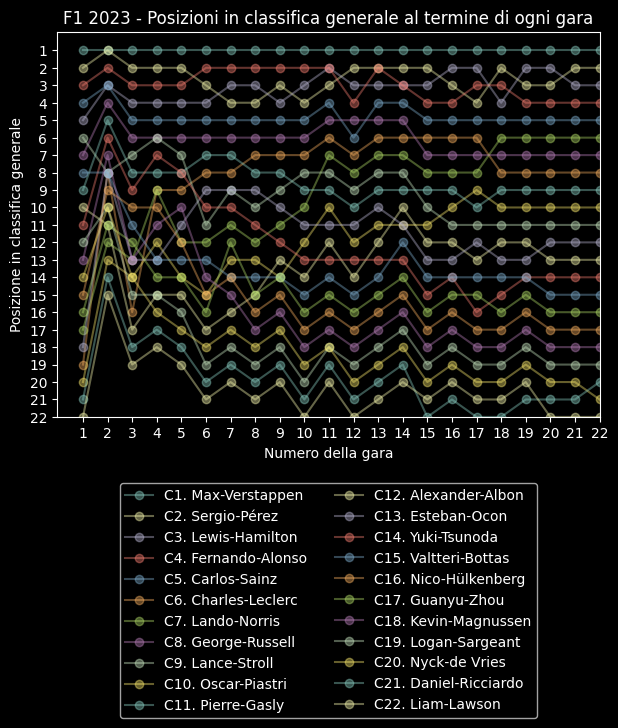
\includegraphics[scale=1.0]{figures/schultzestandings2023.png}
     \caption{Rappresentazione grafica della tabella \ref{table:classifichegeneralischultze} }
 \end{figure}

 \begin{table}[H]
    \centering
    \begingroup
    \resizebox{\linewidth}{!}{%
    \begin{tabular}{|c|c|c|}

    \hline
    \multicolumn{1}{|l|}{Elemento 1} & \multicolumn{1}{l|}{Elemento 2} & \multicolumn{1}{l|}{Valore distanza euclidea} \\ \hline
    Matrice "reale" & Matrice Condorcet &  68.23 \\ \hline
    Matrice "reale" & Matrice Schultze &  44.72 \\ \hline
    Matrice Condorcet & Matrice Schultze &  48.04 \\ \hline
    Classifica finale "reale" & Classifica finale Condorcet &  14.35 \\ \hline
    Classifica finale "reale" & Classifica finale Schultze &  8.31 \\ \hline
    Classifica finale Condorcet & Classifica finale Schultze &  14.04 \\ \hline
    \end{tabular}}
    \endgroup

    \caption{Tabella relativa al Mondiale \textit{\ac{f1}} 2023, in cui per ogni gara (G*)  è riportata la posizione del concorrente (C*) in classifica generale, al termine della gara stessa.
    I valori sono ricavati dall'applicazione dell'algoritmo di Condorcet al termine di ogni gara, considerando anche le precedenti.
    Ogni gara rappresenta un voto, composto dagli ordini di arrivo.
    }
    \label{table:distanzef12023}
\end{table}


%%2008
\begin{table}[H]
    \centering
    \begingroup
    \resizebox{\linewidth}{!}{%
    \begin{tabular}{|c|c|c|c|c|c|c|c|c|c|c|c|c|c|c|c|c|c|c|}

    \hline
    \multicolumn{1}{|l|}{} & \multicolumn{1}{l|}{G1} & \multicolumn{1}{l|}{G2} & \multicolumn{1}{l|}{G3} & \multicolumn{1}{l|}{G4} & \multicolumn{1}{l|}{G5} & \multicolumn{1}{l|}{G6} & \multicolumn{1}{l|}{G7} & \multicolumn{1}{l|}{G8} & \multicolumn{1}{l|}{G9} & \multicolumn{1}{l|}{G10} & \multicolumn{1}{l|}{G11} & \multicolumn{1}{l|}{G12} & \multicolumn{1}{l|}{G13} & \multicolumn{1}{l|}{G14} & \multicolumn{1}{l|}{G15} & \multicolumn{1}{l|}{G16} & \multicolumn{1}{l|}{G17} & \multicolumn{1}{l|}{G18} \\ \hline
    C1. & 8 & 18 & 6 & 4 & 2 & 3 & 3 & 1 & 2 & 2 & 3 & 2 & 2 & 2 & 2 & 2 & 2 & 2 \\ \hline
    C2. & 1 & 1 & 3 & 2 & 3 & 1 & 2 & 4 & 1 & 1 & 1 & 1 & 1 & 1 & 1 & 1 & 1 & 1 \\ \hline
    C3. & 8 & 2 & 1 & 1 & 1 & 2 & 4 & 3 & 3 & 3 & 2 & 3 & 4 & 4 & 4 & 4 & 4 & 3 \\ \hline
    C4. & 8 & 5 & 4 & 3 & 4 & 4 & 1 & 2 & 4 & 4 & 4 & 4 & 3 & 3 & 3 & 3 & 3 & 4 \\ \hline
    C5. & 2 & 3 & 2 & 5 & 5 & 5 & 5 & 5 & 5 & 5 & 5 & 6 & 5 & 5 & 5 & 5 & 5 & 6 \\ \hline
    C6. & 5 & 4 & 5 & 6 & 6 & 6 & 6 & 6 & 6 & 6 & 6 & 5 & 6 & 6 & 6 & 6 & 7 & 7 \\ \hline
    C7. & 4 & 7 & 9 & 10 & 8 & 8 & 9 & 9 & 9 & 9 & 8 & 8 & 8 & 7 & 7 & 7 & 6 & 5 \\ \hline
    C8. & 8 & 8 & 7 & 7 & 9 & 9 & 8 & 7 & 7 & 7 & 7 & 7 & 7 & 8 & 9 & 9 & 9 & 9 \\ \hline
    C9. & 8 & 18 & 14 & 14 & 15 & 17 & 13 & 13 & 14 & 16 & 10 & 10 & 10 & 11 & 10 & 11 & 10 & 10 \\ \hline
    C10. & 8 & 11 & 10 & 8 & 7 & 7 & 7 & 8 & 8 & 8 & 9 & 9 & 9 & 10 & 11 & 10 & 11 & 11 \\ \hline
    C11. & 3 & 6 & 8 & 9 & 10 & 10 & 10 & 10 & 11 & 12 & 13 & 13 & 14 & 14 & 12 & 13 & 13 & 13 \\ \hline
    C12.  & 8 & 18 & 21 & 21 & 22 & 12 & 14 & 14 & 15 & 15 & 16 & 14 & 12 & 9 & 8 & 8 & 8 & 8 \\ \hline
    C13.  & 8 & 12 & 13 & 15 & 14 & 16 & 12 & 12 & 13 & 14 & 15 & 16 & 16 & 16 & 16 & 16 & 16 & 16 \\ \hline
    C14.  & 6 & 9 & 11 & 11 & 11 & 11 & 11 & 11 & 12 & 13 & 14 & 15 & 15 & 15 & 15 & 15 & 15 & 15 \\ \hline
    C15.  & 8 & 16 & 16 & 17 & 17 & 14 & 15 & 15 & 10 & 10 & 12 & 12 & 13 & 13 & 14 & 14 & 14 & 14 \\ \hline
    C16.  & 7 & 10 & 12 & 13 & 13 & 15 & 17 & 18 & 17 & 18 & 18 & 18 & 17 & 17 & 17 & 17 & 17 & 17 \\ \hline
    C17.  & 8 & 14 & 17 & 18 & 18 & 19 & 19 & 17 & 18 & 11 & 11 & 11 & 11 & 12 & 13 & 12 & 12 & 12 \\ \hline
    C18.    & 8 & 13 & 15 & 12 & 12 & 13 & 16 & 16 & 16 & 17 & 17 & 17 & 18 & 18 & 18 & 18 & 18 & 18 \\ \hline
    C19.  & 8 & 15 & 18 & 16 & 16 & 18 & 18 & 19 & 19 & 19 & 19 & 19 & 19 & 19 & 19 & 19 & 19 & 19 \\ \hline
    C20. & 8 & 18 & 21 & 21 & 21 & 22 & 22 & 22 & 22 & 21 & 21 & 21 & 20 & 20 & 20 & 20 & 20 & 20 \\ \hline
    C21. & 8 & 18 & 20 & 19 & 19 & 20 & 20 & 20 & 20 & 20 & 20 & 20 & 21 & 21 & 21 & 21 & 21 & 21 \\ \hline
    C22.  & 8 & 17 & 19 & 20 & 20 & 21 & 21 & 21 & 21 & 22 & 22 & 22 & 22 & 22 & 22 & 22 & 22 & 22 \\ \hline
    \end{tabular}}
    \endgroup
    
    \caption{Tabella relativa al Mondiale \ac{f1} 2008, in cui per ogni gara (G*)  è riportata la posizione del concorrente (C*) in classifica generale, al termine della gara stessa.
    I valori sono ricavati da Ergast API \cite{WebsiteErgastAPIStandings}}
    \label{table:classifichegeneralireali2008}
\end{table}

\begin{figure}[H]
    \centering
     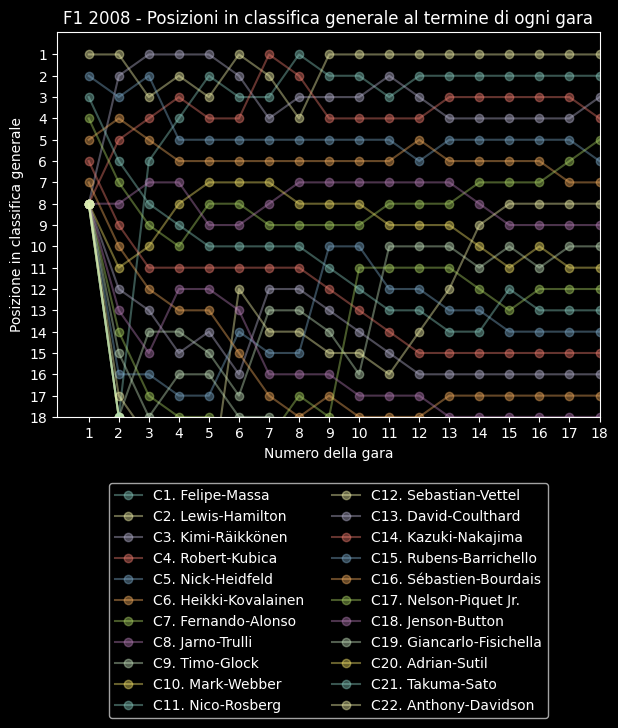
\includegraphics[scale=1.0]{figures/realstandings2008.png}
     \caption{Rappresentazione grafica della tabella \ref{table:classifichegeneralireali} }
 \end{figure}


 \begin{table}[H]
    \centering
    \begingroup
    \resizebox{\linewidth}{!}{%
    \begin{tabular}{|c|c|c|c|c|c|c|c|c|c|c|c|c|c|c|c|c|c|c|}

    \hline
    \multicolumn{1}{|l|}{} & \multicolumn{1}{l|}{G1} & \multicolumn{1}{l|}{G2} & \multicolumn{1}{l|}{G3} & \multicolumn{1}{l|}{G4} & \multicolumn{1}{l|}{G5} & \multicolumn{1}{l|}{G6} & \multicolumn{1}{l|}{G7} & \multicolumn{1}{l|}{G8} & \multicolumn{1}{l|}{G9} & \multicolumn{1}{l|}{G10} & \multicolumn{1}{l|}{G11} & \multicolumn{1}{l|}{G12} & \multicolumn{1}{l|}{G13} & \multicolumn{1}{l|}{G14} & \multicolumn{1}{l|}{G15} & \multicolumn{1}{l|}{G16} & \multicolumn{1}{l|}{G17} & \multicolumn{1}{l|}{G18}  \\ \hline
    C1.  & 13 & 12 & 8 & 6 & 2 & 2 & 1 & 1 & 1 & 1 & 1 & 1 & 1 & 1 & 1 & 1 & 1 & 1 \\ \hline
    C2.  & 1 & 1 & 4 & 3 & 3 & 1 & 2 & 3 & 3 & 2 & 1 & 2 & 2 & 2 & 2 & 1 & 2 & 2 \\ \hline
    C3.  & 8 & 4 & 1 & 1 & 1 & 1 & 1 & 1 & 2 & 2 & 1 & 3 & 3 & 5 & 5 & 4 & 3 & 3 \\ \hline
    C4.  & 9 & 5 & 2 & 2 & 4 & 2 & 3 & 2 & 4 & 3 & 2 & 3 & 3 & 3 & 3 & 2 & 3 & 3 \\ \hline
    C5.  & 2 & 2 & 3 & 3 & 5 & 3 & 4 & 3 & 5 & 4 & 3 & 4 & 4 & 4 & 3 & 3 & 4 & 4 \\ \hline
    C6.  & 5 & 3 & 3 & 4 & 9 & 5 & 5 & 4 & 6 & 5 & 4 & 4 & 5 & 4 & 4 & 3 & 5 & 5 \\ \hline
    C7.  & 4 & 5 & 6 & 5 & 8 & 6 & 9 & 6 & 9 & 8 & 7 & 7 & 8 & 7 & 6 & 5 & 6 & 6 \\ \hline
    C8.  & 15 & 7 & 4 & 4 & 6 & 6 & 6 & 4 & 7 & 6 & 5 & 5 & 6 & 6 & 7 & 6 & 7 & 7 \\ \hline
    C9. & 10 & 13 & 7 & 7 & 11 & 8 & 11 & 8 & 11 & 10 & 9 & 9 & 9 & 8 & 9 & 8 & 9 & 8 \\ \hline
    C10.  & 17 & 9 & 5 & 4 & 7 & 4 & 7 & 5 & 8 & 7 & 6 & 6 & 7 & 7 & 8 & 7 & 8 & 8 \\ \hline
    C11.  & 3 & 6 & 5 & 6 & 7 & 7 & 8 & 7 & 10 & 9 & 8 & 8 & 10 & 9 & 10 & 9 & 10 & 9 \\ \hline
    C12.  & 20 & 13 & 16 & 13 & 19 & 14 & 19 & 14 & 16 & 13 & 13 & 13 & 13 & 11 & 12 & 10 & 10 & 9 \\ \hline
    C13.  & 14 & 8 & 9 & 8 & 12 & 9 & 12 & 7 & 12 & 10 & 10 & 10 & 11 & 10 & 11 & 11 & 11 & 10 \\ \hline
    C14. & 6 & 9 & 7 & 7 & 11 & 8 & 11 & 10 & 11 & 10 & 11 & 12 & 12 & 11 & 12 & 12 & 12 & 11 \\ \hline
    C15.  & 22 & 13 & 12 & 9 & 13 & 10 & 13 & 8 & 13 & 10 & 11 & 11 & 12 & 13 & 14 & 14 & 12 & 11 \\ \hline
    C16.  & 7 & 13 & 9 & 10 & 14 & 13 & 16 & 12 & 15 & 13 & 13 & 13 & 13 & 13 & 14 & 14 & 13 & 12 \\ \hline
    C17.  & 12 & 8 & 10 & 11 & 16 & 11 & 14 & 11 & 15 & 12 & 12 & 12 & 13 & 13 & 15 & 14 & 10 & 12 \\ \hline
    C18. & 18 & 10 & 15 & 11 & 10 & 8 & 10 & 9 & 14 & 11 & 11 & 11 & 12 & 12 & 13 & 13 & 14 & 12 \\ \hline
    C19.  & 21 & 12 & 11 & 8 & 13 & 12 & 15 & 12 & 16 & 14 & 14 & 14 & 14 & 14 & 16 & 15 & 15 & 13 \\ \hline
    C20.  & 16 & 13 & 14 & 12 & 18 & 13 & 17 & 13 & 16 & 15 & 15 & 15 & 15 & 15 & 17 & 16 & 16 & 14 \\ \hline
    C21. & 11 & 11 & 13 & 10 & 15 & 12 & 16 & 13 & 17 & 16 & 16 & 16 & 16 & 16 & 18 & 17 & 17 & 15 \\ \hline
    C22.  & 19 & 12 & 13 & 11 & 17 & 13 & 18 & 14 & 18 & 17 & 17 & 17 & 17 & 17 & 19 & 18 & 18 & 16 \\ \hline
    \end{tabular}}
    \endgroup
  
    \caption{Tabella relativa al Mondiale \ac{f1} 2008, in cui per ogni gara (G*)  è riportata la posizione del concorrente (C*) in classifica generale, al termine della gara stessa.
    I valori sono ricavati dall'applicazione dell'algoritmo di Condorcet al termine di ogni gara, considerando anche le precedenti.
    Ogni gara rappresenta un voto, composto dagli ordini di arrivo.
    }
    \label{table:classifichegeneralicondorcet2008}
\end{table}

\begin{figure}[H]
    \centering
     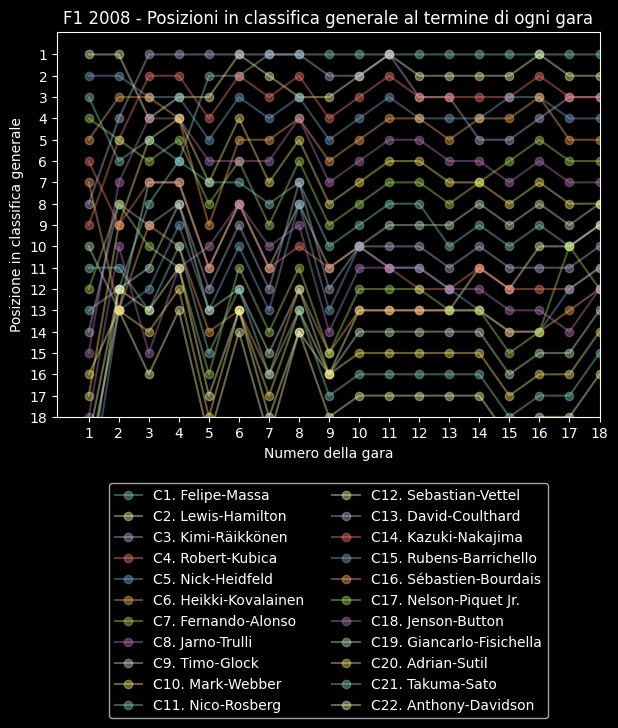
\includegraphics[scale=1.0]{figures/condorcetstandings2008.png}
     \caption{Rappresentazione grafica della tabella \ref{table:classifichegeneralicondorcet} }
 \end{figure}


\begin{table}[H]
    \centering
    \begingroup
    \resizebox{\linewidth}{!}{%
    \begin{tabular}{|c|c|c|c|c|c|c|c|c|c|c|c|c|c|c|c|c|c|c|}

    \hline
    \multicolumn{1}{|l|}{} & \multicolumn{1}{l|}{G1} & \multicolumn{1}{l|}{G2} & \multicolumn{1}{l|}{G3} & \multicolumn{1}{l|}{G4} & \multicolumn{1}{l|}{G5} & \multicolumn{1}{l|}{G6} & \multicolumn{1}{l|}{G7} & \multicolumn{1}{l|}{G8} & \multicolumn{1}{l|}{G9} & \multicolumn{1}{l|}{G10} & \multicolumn{1}{l|}{G11} & \multicolumn{1}{l|}{G12} & \multicolumn{1}{l|}{G13} & \multicolumn{1}{l|}{G14} & \multicolumn{1}{l|}{G15} & \multicolumn{1}{l|}{G16} & \multicolumn{1}{l|}{G17} & \multicolumn{1}{l|}{G18}  \\ \hline
    C1.  & 13 & 14 & 9 & 7 & 5 & 3 & 3 & 3 & 5 & 4 & 6 & 5 & 3 & 3 & 4 & 4 & 4 & 3 \\ \hline
    C2.  & 1 & 1 & 5 & 4 & 3 & 2 & 3 & 4 & 3 & 3 & 3 & 2 & 1 & 2 & 1 & 2 & 1 & 1 \\ \hline
    C3.  & 8 & 3 & 1 & 1 & 1 & 1 & 2 & 2 & 2 & 2 & 1 & 3 & 6 & 6 & 6 & 6 & 5 & 5 \\ \hline
    C4.  & 9 & 4 & 4 & 2 & 2 & 1 & 1 & 1 & 1 & 1 & 2 & 1 & 2 & 1 & 2 & 1 & 2 & 2 \\ \hline
    C5.  & 2 & 2 & 2 & 3 & 4 & 4 & 2 & 5 & 4 & 4 & 4 & 6 & 4 & 4 & 3 & 3 & 3 & 4 \\ \hline
    C6.  & 5 & 2 & 3 & 5 & 6 & 6 & 4 & 6 & 6 & 5 & 5 & 4 & 5 & 5 & 5 & 5 & 7 & 7 \\ \hline
    C7.  & 4 & 5 & 6 & 9 & 7 & 7 & 6 & 8 & 9 & 7 & 8 & 9 & 8 & 8 & 7 & 7 & 6 & 6 \\ \hline
    C8.  & 15 & 7 & 7 & 6 & 7 & 8 & 5 & 7 & 7 & 6 & 7 & 7 & 7 & 7 & 8 & 8 & 8 & 8 \\ \hline
    C9.  & 10 & 13 & 11 & 12 & 11 & 11 & 8 & 10 & 11 & 10 & 11 & 11 & 10 & 10 & 10 & 11 & 10 & 10 \\ \hline
    C10. & 17 & 9 & 8 & 8 & 7 & 5 & 4 & 7 & 8 & 7 & 9 & 8 & 9 & 9 & 9 & 9 & 9 & 9 \\ \hline
    C11.  & 3 & 6 & 7 & 10 & 8 & 9 & 7 & 9 & 10 & 8 & 10 & 10 & 11 & 11 & 11 & 10 & 11 & 11 \\ \hline
    C12.  & 20 & 19 & 20 & 20 & 19 & 19 & 14 & 16 & 18 & 15 & 17 & 16 & 17 & 14 & 13 & 12 & 12 & 12 \\ \hline
    C13.  & 14 & 8 & 12 & 13 & 9 & 13 & 9 & 11 & 14 & 12 & 13 & 13 & 13 & 13 & 13 & 14 & 15 & 15 \\ \hline
    C14.  & 6 & 8 & 10 & 11 & 10 & 10 & 10 & 12 & 13 & 9 & 12 & 12 & 12 & 12 & 12 & 13 & 13 & 13 \\ \hline
    C15.  & 22 & 17 & 16 & 16 & 14 & 14 & 12 & 13 & 12 & 11 & 14 & 14 & 15 & 16 & 15 & 16 & 17 & 17 \\ \hline
    C16.  & 7 & 12 & 14 & 17 & 16 & 18 & 15 & 18 & 17 & 16 & 18 & 17 & 18 & 18 & 16 & 17 & 18 & 18 \\ \hline
    C17.  & 12 & 8 & 13 & 17 & 15 & 16 & 14 & 15 & 16 & 13 & 15 & 13 & 14 & 15 & 14 & 14 & 14 & 14 \\ \hline
    C18.  & 18 & 11 & 17 & 14 & 12 & 12 & 11 & 14 & 15 & 14 & 16 & 15 & 16 & 17 & 14 & 15 & 16 & 16 \\ \hline
    C19.  & 21 & 15 & 15 & 14 & 13 & 15 & 13 & 17 & 17 & 17 & 19 & 18 & 19 & 19 & 17 & 18 & 19 & 19 \\ \hline
    C20. & 16 & 18 & 19 & 19 & 18 & 20 & 17 & 20 & 20 & 18 & 20 & 19 & 20 & 20 & 18 & 19 & 20 & 20 \\ \hline
    C21.  & 11 & 10 & 14 & 15 & 15 & 17 & 16 & 19 & 19 & 19 & 21 & 20 & 21 & 21 & 19 & 20 & 21 & 21 \\ \hline
    C22.  & 19 & 16 & 18 & 18 & 17 & 21 & 18 & 21 & 21 & 20 & 22 & 21 & 22 & 22 & 20 & 21 & 22 & 22 \\ \hline
    \end{tabular}}
    \endgroup

    \caption{Tabella relativa al Mondiale \textit{\ac{f1}} 2008, in cui per ogni gara (G*)  è riportata la posizione del concorrente (C*) in classifica generale, al termine della gara stessa.
    I valori sono ricavati dall'applicazione dell'algoritmo di Schultze al termine di ogni gara, considerando anche le precedenti.
    Ogni gara rappresenta un voto, composto dagli ordini di arrivo.
    }
    \label{table:classifichegeneralischultze2008}
\end{table}

\begin{figure}[H]
    \centering
     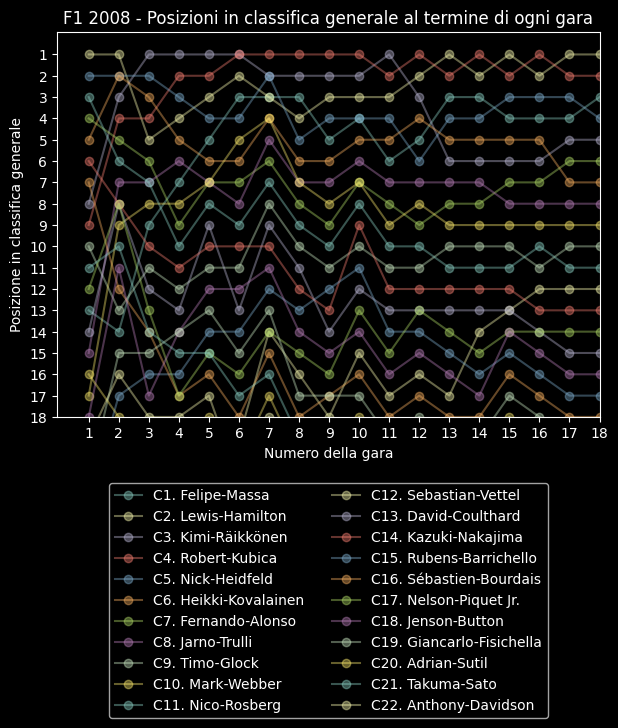
\includegraphics[scale=1.0]{figures/schultzestandings2008.png}
     \caption{Rappresentazione grafica della tabella \ref{table:classifichegeneralischultze} }
 \end{figure}

 \begin{table}[H]
    \centering
    \begingroup
    \resizebox{\linewidth}{!}{%
    \begin{tabular}{|c|c|c|}

    \hline
    \multicolumn{1}{|l|}{Elemento 1} & \multicolumn{1}{l|}{Elemento 2} & \multicolumn{1}{l|}{Valore distanza euclidea} \\ \hline
    Matrice "reale" & Matrice Condorcet &  77.19 \\ \hline
    Matrice "reale" & Matrice Schultze &  52.53 \\ \hline
    Matrice Condorcet & Matrice Schultze &  55.94 \\ \hline
    Classifica finale "reale" & Classifica finale Condorcet &  24.6 \\ \hline
    Classifica finale "reale" & Classifica finale Schultze &  12.45 \\ \hline
    Classifica finale Condorcet & Classifica finale Schultze &  19.34 \\ \hline
    \end{tabular}   }
    \endgroup

    \caption{Tabella relativa al Mondiale \textit{\ac{f1}} 2008, in cui per ogni gara (G*)  è riportata la posizione del concorrente (C*) in classifica generale, al termine della gara stessa.
    I valori sono ricavati dall'applicazione dell'algoritmo di Condorcet al termine di ogni gara, considerando anche le precedenti.
    Ogni gara rappresenta un voto, composto dagli ordini di arrivo.
    }
    \label{table:distanzef12008}
\end{table}
%----------------------------------------------------------------------------------------
\chapter{Conclusioni}




%Write your intro here.
%\sidenote{Add sidenotes in this way. They are named after the author of the thesis}

%You can use acronyms that your defined previously,
%You can use acronyms that your defined previously,
%such as \ac{IoT}.
%
%If you use acronyms twice,
%they will be written in full only once
%(indeed, you can mention the \ac{IoT} now without it being fully explained).
%
%In some cases, you may need a plural form of the acronym.
%
%For instance,
%that you are discussing \acp{vm},
%you may need both \ac{vm} and \acp{vm}.

%\paragraph{Structure of the Thesis}

%\note{At the end, describe the structure of the paper}

%\chapter{State of the art}

%I suggest referencing stuff as follows: \cref{fig:random-image} or \Cref{fig:random-image}

%\begin{figure}
%    \centering
%    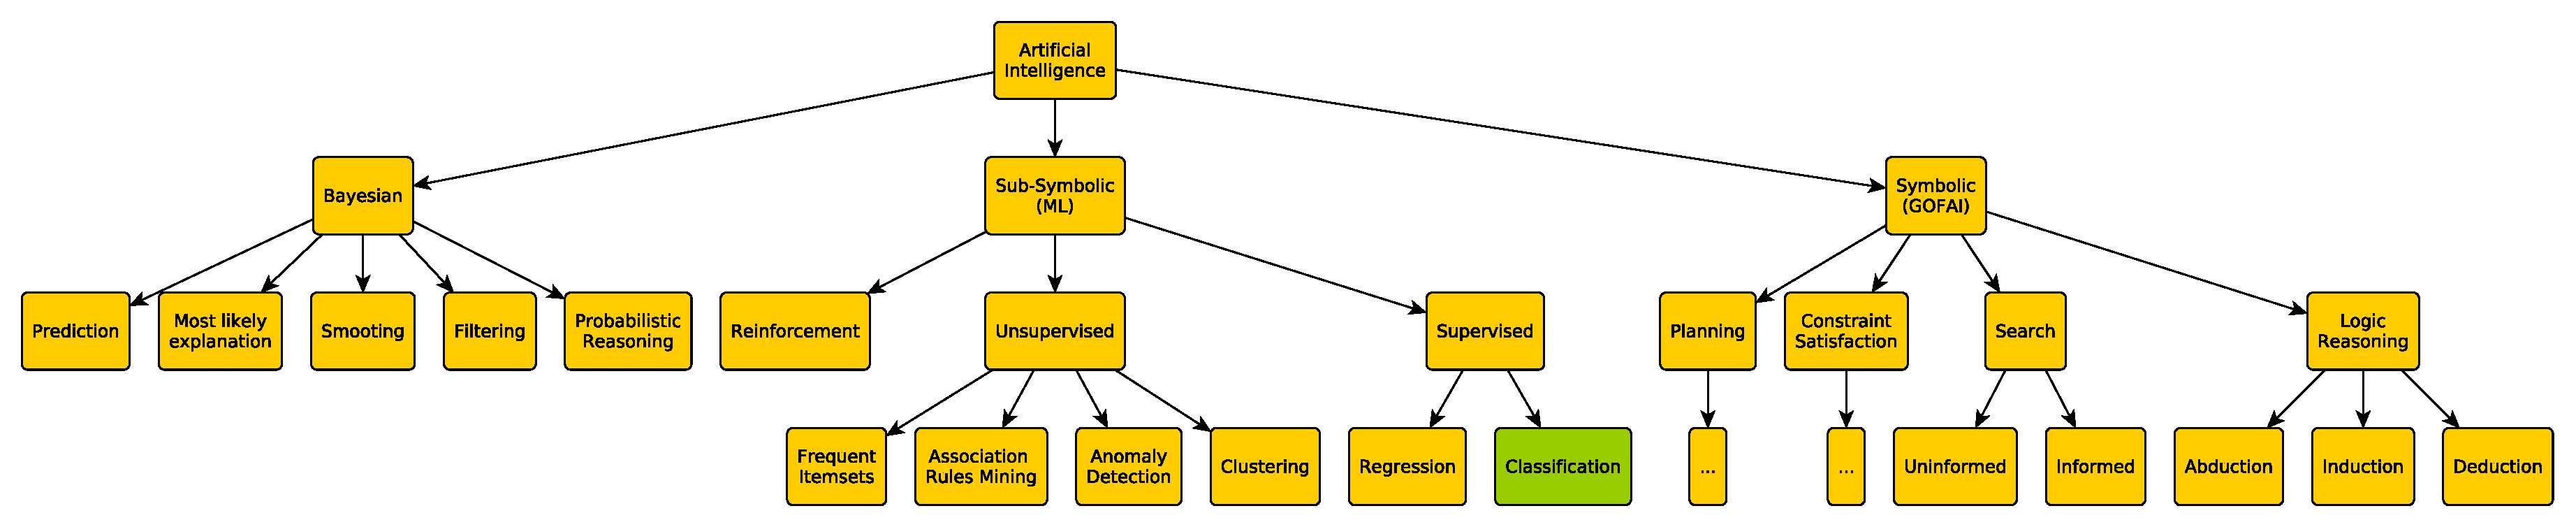
\includegraphics[width=.8\linewidth]{figures/random-image.pdf}
%    \caption{Some random image}
%    \label{fig:random-image}
%\end{figure}

%\section{Some cool topic}

%\chapter{Contribution}

%You may also put some code snippet (which is NOT float by default), eg: \cref{lst:random-code}.

%\lstinputlisting[float,language=Java,label={lst:random-code}]{listings/HelloWorld.java}

%\section{Fancy formulas here}

%----------------------------------------------------------------------------------------
% BIBLIOGRAPHY
%----------------------------------------------------------------------------------------

\backmatter

\nocite{*} % comment this to only show the referenced entries from the .bib file


\bibliographystyle{alpha}
\bibliography{bibliography}

\end{document}